\chapter{Above threshold ionization in laser-atom and laser-molecule interactions}
\label{cha:ati}

% -ATI models, keldysh approach pionnering work with the strong field
% approximation
% -QM generalization including rescattering
% -study of the ATI spectrum following the one introduced by kopold

Generally, the interaction of an atom with intense laser fields is
associated with photoionization of the atom by the absorption of one
or more photons. In fact, in very intense laser fields an atom may
absorb many more photons than the minimum required to get ionized,
ejecting an electron of very high energy. The photoelectron energy
spectrum associated with this effect exhibits a series of peaks
separated by the energy of a laser photon. This phenomenon is known as
above threshold ionization (ATI) and was first observed by
Agostini et al~\cite{ATI1979}.

ATI has been tackled by means of diverse approaches, with analytical
approximations dating back to the Keldysh theory which represents a
strong-field approximation~\cite{KeldyshSFA}. Alternatively, attempts
to find a numerical solution to the time-dependent Schr\"{o}dinger
equation (TDSE)~\cite{muller_tdse1999, scrinzi_tdse1999, Joachain2000}
have been instrumental for the understanding of ATI, and a variety of
efforts that deal with the complexity of solving this challenging
numerical problem have been successful in the
past~\cite{Becker_ati2002}. In the same way, complementary approaches
to the solution of the TDSE, such as the so-called Volkov-state
methods~\cite{Faisal_1973, Reiss_1980, Kaminski_1997}, have revealed
their strengths within strong-laser field problems in which a
numerical solution would involve a computationally taxing problem. The
strong-field approximation~\cite{KeldyshSFA}, which treats the binding
potential of the atom as a perturbation once the electron has been
promoted into the continuum where the external laser field governs the
electron dynamics, is the foundation to the formalism discussed in
this chapter.

Sec.~\ref{sec:keldysh} presents an overview of the pioneering work by
Keldysh to describe the laser ionization of atoms. Next, a generalized
approach that introduces rescattering of the electron back to the
vicinity of the binding potential is included in
Sec.~\ref{kopold_sfa}. The ionization regime of a model He atom under
a strong-laser field is explored in Sec.~\ref{sec:kopold_qm} for both
scenarios: considering only direct electrons where the ionization
spectrum is reproduced by the Keldysh amplitude, and using a compact
expression for the transition amplitude that encloses the limiting
case of direct trajectories while allowing electrons to rescatter to
the parent ion as well. Additionally, this study is extended to
explore the laser ionization of the $1b_{1}$ and $1b_{2}$ molecular
orbitals of H$_{2}$O in Sec.~\ref{sec:mo_sfa}. The analysis presented
in this chapter closely follows that of~\cite{Kopold_1997sfa}.



%In addiion to exploring the ionization regime of the He atom in
%Sec.~\ref{sec:kopold_qm}, laser ionization of the $1b_{1}$ and
%$1b_{2}$ molecular orbitals of H$_{2}$O is discussed in
%Sec.~\ref{sec:mo_sfa}.

\section{\label{sec:mpi&tunneling} Multiphoton versus tunneling ionization}

As a result of the interaction with strong laser pulses that compete
with the Coulomb forces, the electron dynamics in atoms and molecules
is characterized by multiphoton processes that determine their
response to the laser field. The Keldysh theory of strong-field
approximation illustrates how the dynamics of the underlying phenomena
that contribute to the formation of ionization spectrum evolves as the
laser field intensity increases~\cite{KeldyshSFA}.

% explain MPI from review papers
% reference fig:mpi_tunneling
% ADD TYPICAL BINDING ENERGY OF THE OUTER (VALENCE) ELECTRONS
% ADD TYPICAL PHOTON ENERGIES
At moderate intensities, $I < 10^{14}\ \mathrm{W/cm^{2}}$, atomic
states undergo a transition from bound states into the continuum due
to the multiphoton excitation linked to the interaction with the laser
field, this phenomenon is known as multiphoton ionization (MPI). The
interaction with intense laser fields induces an ac Stark shift of the
atomic bound states that is responsible for the peak suppression in
the ionization spectrum as the field intensity
increases~\cite{MullerStark_1988}. While states near the nucleus have
a negligible shift in energy due their strong bond and are, in fact,
harder to influence by the field, the upward shift of the higher
states and continuum can become appreciable in the form of an increase
in the ionization potential of the atom, see
Figure~\ref{fig:mpi_tunneling}(a). This shift is given by the electron
ponderomotive energy, $U_{p} = e^{2}E^{2} / 4m\omega^{2}$, which is
the cycle-averaged kinetic energy of a free electron in the electric
field of strength $E$ and frequency $\omega$. Although this increase
in the ionization potential could, possibly, make some transitions
energetically forbiden, in a smoothly varying pulse ionization
channels may not be closed for the entire pulse, in such a way that
the corresponding peak in the ionization spectrum will not vanish
completely~\cite{Protopapas_mpi_tunneling,Joachain_mpi_tunneling}.
%For strong laser fields, $U_{p}$ may become quite large, of the order
%of several $\mathrm{eV}$, causing many states to shift through
%resonance as their energies change, during a laser pulse, by an
%amount larger than the incident photon energy.

At sufficiently high intensity, $I > 10^{14}\ \mathrm{W/cm^2}$, and
low frequency, the ionization process is ruled by a tunneling
mechanism. In this regime, ionization can be described by means of a
quasi-static approach in which, in the low-frequency limit, as the
laser field intensity approaches the Coulomb binding potential of the
ion core, the bound electrons experience an effective potential that
results from the interaction between the laser electric field and the
Coulomb attraction from the ion core~\cite{KeldyshSFA}. This effective
potential acts as an oscillating barrier through which electrons can
escape via tunneling, as Figure~\ref{fig:mpi_tunneling}(b)
illustrates. In the tunneling regime, since the laser field varies
slowly compared to the response time of the electron, the ionization
rate becomes the cycle average of the instantaneous dc tunneling
rate. A fundamental quantity in Keldysh theory, known as Keldysh
parameter, is the ratio of the incident laser frequency to the
tunneling rate, and can be written as~\cite{KeldyshSFA}
%
\begin{eqnarray}
\begin{split}
\gamma = \frac{\omega}{\omega_{t}} & = & \sqrt{\frac{I_{p}}{2 U_{p}}},
\end{split}
\end{eqnarray}
%
where $I_{p}$ is the field-free atomic ionization potential. The
Keldysh parameter illustrates the limits of applicability of the
competing mechanisms that characterize the ionization process. For
$\gamma < 1$, tunneling dynamics will dominate, whereas for $\gamma >
1$ multiphoton dynamics will prevail. In this chapter, we will refer
to the tunneling regime as it is one of the fundamental processes in
ATI.

\begin{figure}
  \centering
  \begin{subfigure}[b]{0.5\linewidth}
    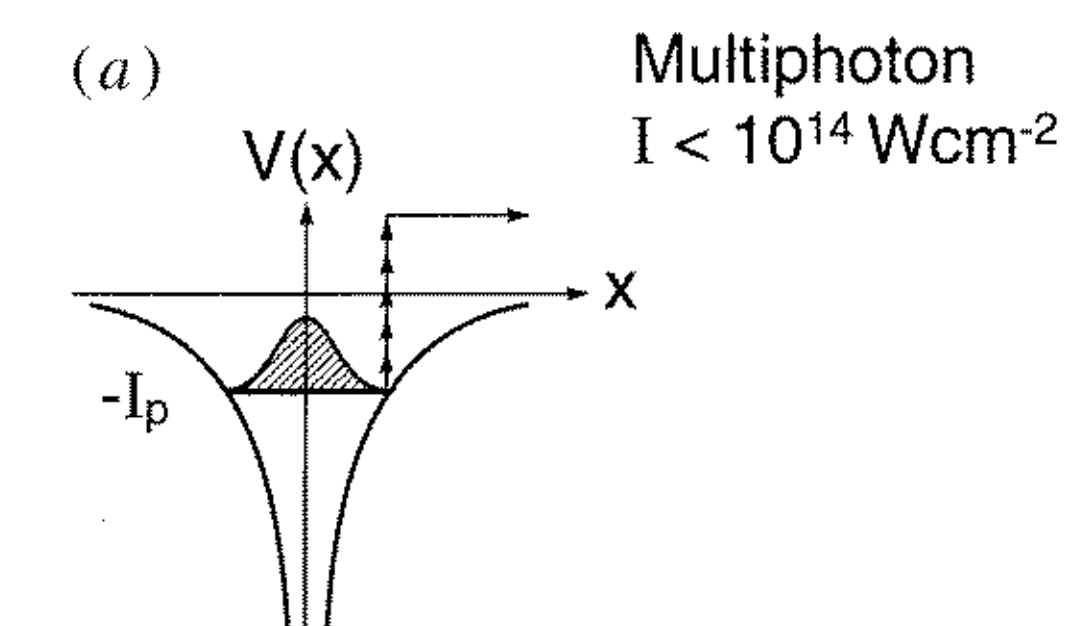
\includegraphics[width=\textwidth]{figures/ch_ATI_SFA/multiphoton}
  \end{subfigure}
  \centering
  \begin{subfigure}[b]{0.46\linewidth}
    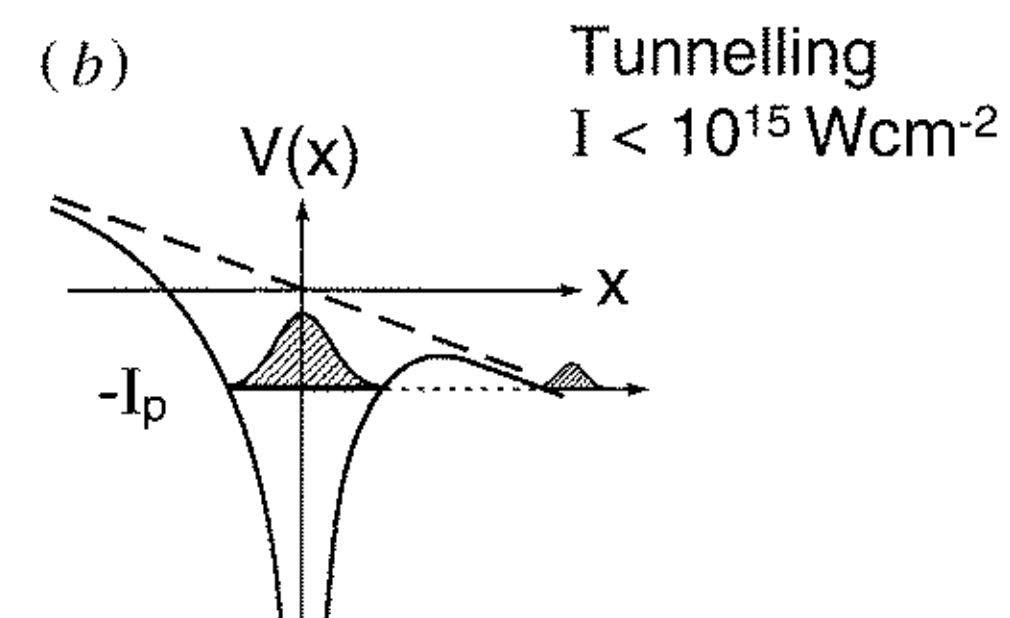
\includegraphics[width=\textwidth]{figures/ch_ATI_SFA/tunneling}
  \end{subfigure}  
  \caption{Schematic representation of (a) multiphoton ionization and
    (b) tunneling ionization as the laser intensity, $I$,
    increases. The dashed line corresponds to the contribution to the
    potential energy due to the instantaneous laser electric
    field. The solid line represents the full effective
    potential. From Ref.~\cite{Protopapas_mpi_tunneling}.}
  \label{fig:mpi_tunneling}
\end{figure}


\section{\label{sec:keldysh} Keldysh formalism}
% explain a little bit more the plateau, origin etc,
% use illustration from literature (PRL72_Paulus)

Even though the Keldysh formalism for strong-field ionization provided
very good agreement with experimental data of electron ATI spectra for
helium ionization~\cite{Walker_1994exp}, rescattering effects were not
included in the theory and it failed to reproduce the rescattering
induced plateau that is visible in measurements along a broad energy
spectrum~\cite{Paulus_1994plateau, Walker_1996}, and emerged as a
prevalent feature in the ATI energy
spectrum. Figure~\ref{fig:plateau_ATI} shows the presence of such
plateau as a marked change of slope in the ionization spectrum of rare
gases. A recollision picture in which the strong-field ionization is
characterized by several steps, involving tunneling of the electron
followed by a free interaction with the laser field in which the
electron returns to the core, was introduced later
on~\cite{Corkum_1993, LewensteinSPA_1994}. In this chapter we are
concerned with the numerical evaluation of an improved Keldysh
approximation~\cite{Kopold_1997sfa} that accounts for rescattering
effects and reveals the complex structure of the ionization spectrum.

\begin{figure}
  \centering
  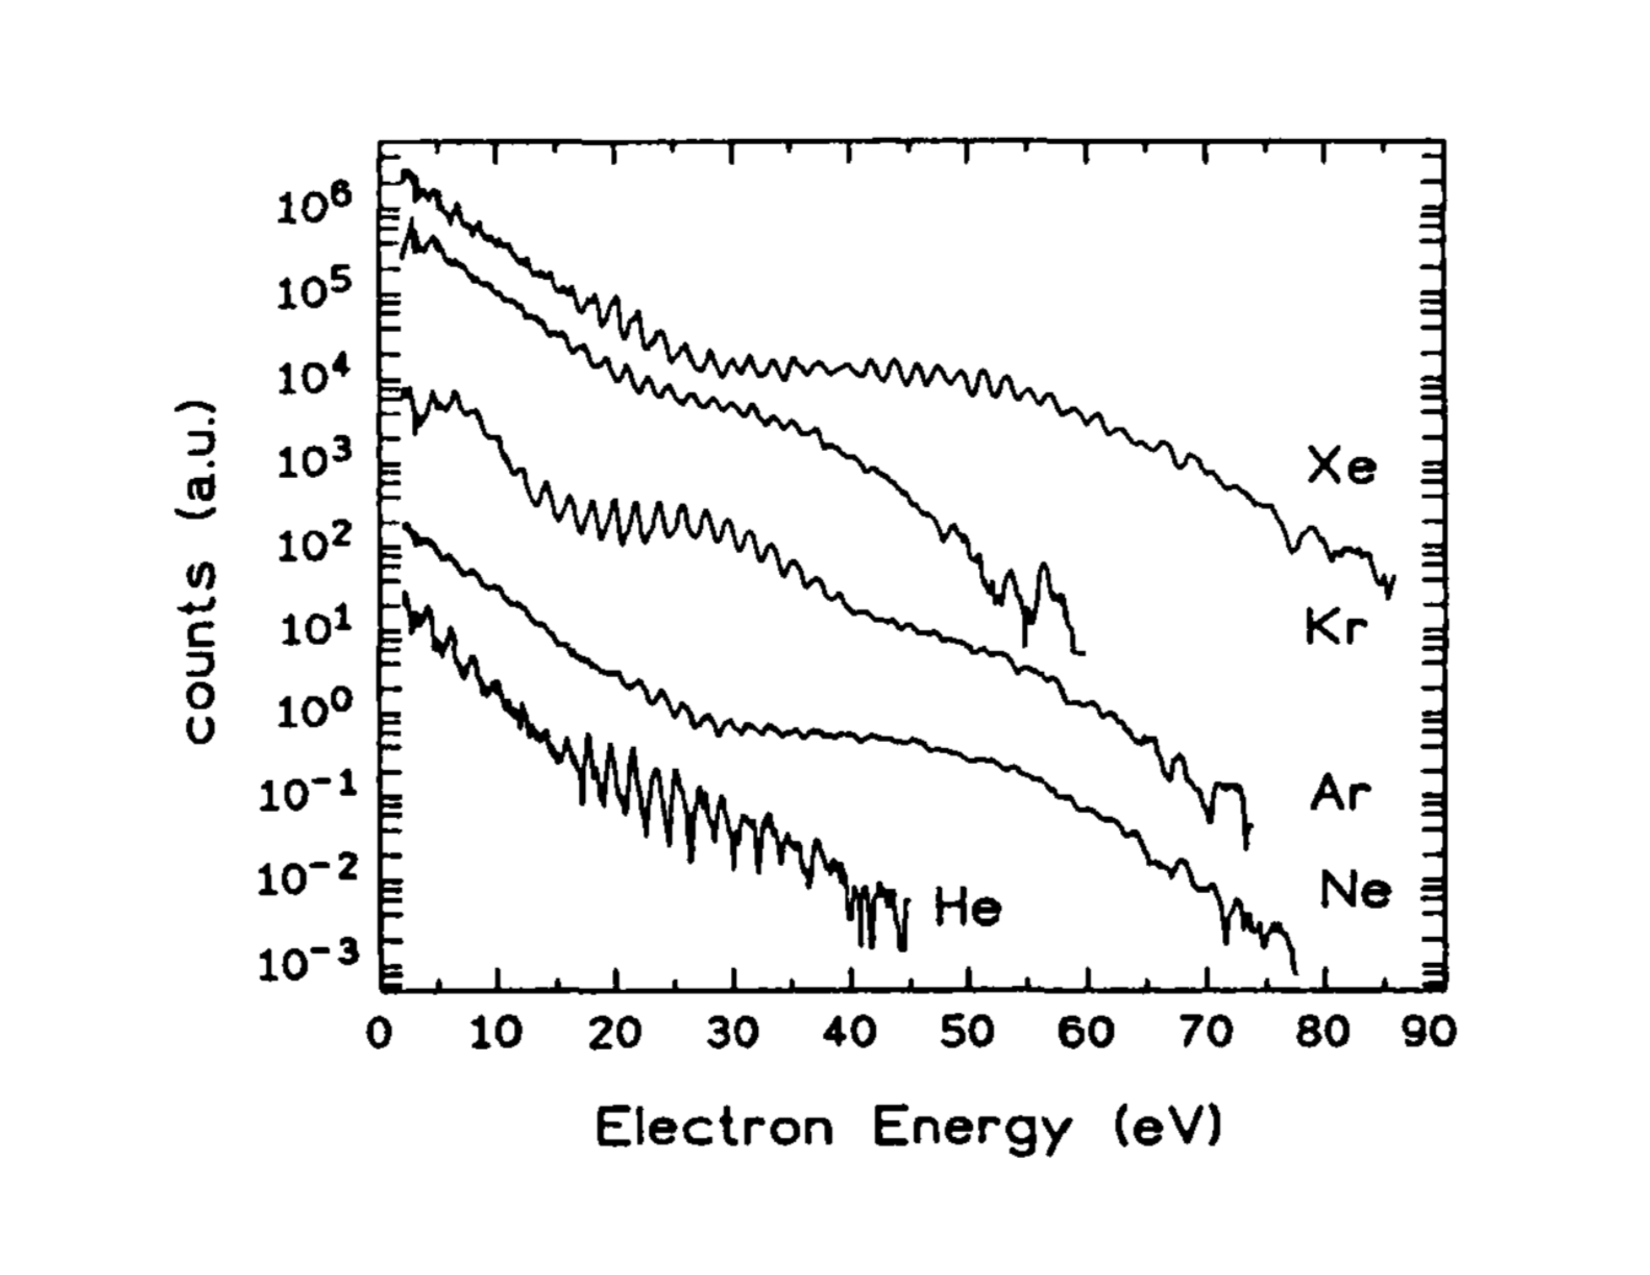
\includegraphics[width=0.75\textwidth]{figures/ch_ATI_SFA/plateauPRL72}
  \caption{ATI spectra for various noble gases, at a wavelength of
    $\lambda = 630\ \rm{nm}$ and an intensity of $I \simeq 2\times
    10^{14}\ \rm{W/cm^{2}}$ ($3\times 10^{14}\ \rm{W/cm^{2}}$ for
    He). From Ref.~\cite{Paulus_1994plateau}}
  \label{fig:plateau_ATI}
\end{figure}

The probability amplitude for an electron to transfer from the ground
state of an atom with binding potential $V(\mathbf{r})$ into a
scattering state $|\psi_{\mathbf{p}}(t)\rangle$ due to an external
laser field is given by~\cite{Kopold_1997sfa}
\begin{eqnarray}
\label{eq:matrix_element}
\begin{split}
M_{\mathbf{p}} & = & \lim_{t\to\infty,t'\to -\infty}
{\langle \psi_{\mathbf{p}}(t) | U(t,t') | \psi_{0}(t') \rangle},
\end{split}
\end{eqnarray}
where it is assumed that in the limit of early times, $t'\to -\infty$,
the exact wave function reduces to the unperturbed wave function
$\psi_{0}(t)$ of the initial ground state. In order to express the
total wave function in terms of the unperturbed wave function, the
evolution operator formalism~\cite{BeckerTEOp_2006} is
implemented. The time-evolution operator, $U(t,t')$, propagates the
wave function $|\psi(t)\rangle$ from $t'$ to $t$ under the full
Hamiltonian
\begin{eqnarray}
\label{eq:H_ati}
\begin{split}
H(t) & = & -\frac{1}{2} \nabla^{2} + H_{I}(t) + V(\mathbf{r}),
\end{split}
\end{eqnarray}
which includes the binding potential of the parent ion,
$V(\mathbf{r})$, and the interaction with the laser field,
$H_{I}(t)=-\mathbf{r}\cdot\mathbf{E}(t)$, under the dipole
approximation in the length gauge~\cite{Kopold_1997sfa}.

The time-evolution operator satisfies an integral equation, namely the
Dyson equation~\cite{Kopold_1997sfa, cjp2010_keldysh}, which
conveniently allows to construct an expansion in which the interaction
with the external field is treated as a perturbation. This
representation, together with the orthogonality of the initial ground
state $|\psi_{0}\rangle$ and scattering state
$|\psi_{\mathbf{p}}\rangle$, illustrates the possibility of major
excursions of the scattering electron away from its parent ion once it
was propagated from the initial state by $U(t,t')$.

Two approximations are crucial to derive the Keldysh result for the
transition amplitude~\cite{Kopold_1997sfa}. The first approximation
consists of replacing the complete time-evolution operator
in~(\ref{eq:matrix_element}) by the Volkov time-evolution operator
$U^{V}(t,t')$, which propagates the wave function of a free electron
coupled through the interaction $H_{I}(t)$ to the external laser
field. In other words, the interaction with the binding potential is
considered a perturbation everywhere except in the initial and final
states. In the second approximation the scattering state,
$\psi_{\mathbf{p}}$, is replaced by the Volkov wave function,
$\psi_{\mathbf{p}}^{(V)}$, which represents the state of a free
electron in a laser field with time-averaged momentum
$\mathbf{p}$. Further details about the derivation are to be found
in~\cite{Kopold_1997sfa}. These transformations, along with additional
algebraic operations, lead to obtain an equivalent form of the
standard Keldysh amplitude~\cite{Kopold_1997sfa, Becker_1997}
\begin{eqnarray}
\label{eq:keldysh_amp}
\begin{split}
M_{\mathbf{p}}^{(0)} & = &
-i \int\limits_{-\infty}\limits^{\infty}
dt\ \langle \psi_{\mathbf{p}}^{(V)}(t) | V | \psi_{0}(t) \rangle.
\end{split}
\end{eqnarray}

Generally, replacing the time-evolution propagator $U(t,t')$ by the
Volkov propagator $U^{(V)}(t,t')$ is more justified the shorter the
range of the binding potential and the higher the intensity of the
laser field. In what follows, we will consider the limiting case of
zero-range interactions of the form
%
\begin{eqnarray}
\label{eq:zero-range}
\begin{split}
V(\mathbf{r}) & = & -\lambda\ \delta(\mathbf{r})
%V(\mathbf{r}) & = & \frac{2\pi}{m\mathbf{\kappa}}
%\delta(\mathbf{r}) \frac{\partial}{\partial r} r,
\end{split}
\end{eqnarray}
%
which has a bound state or more depending on
$\lambda$~\cite{Becker_rescattering1994, Becker_ati2002}. Zero-range
potentials have been widely used in tunneling~\cite{Kleber_zeroV1994}
and multiphoton ionization problems~\cite{Becker_zeroV1990}, as well
as to simulate the electron dynamics in molecular systems under
intense laser fields~\cite{frolov_zeroV2013}. Inserting the zero-range
potential~(\ref{eq:zero-range}) into the Keldysh
amplitude~(\ref{eq:keldysh_amp}) yields the expansion
%
\begin{eqnarray}
\label{eq:keldysh_amp_explicit}
\begin{split}
M_{\mathbf{p}}^{(0)} \sim &
\frac{m}{2\pi}\sqrt{2m|E_{0}|}
\sum\limits_{n} \delta\left(\frac{p^{2}}{2m} + U_{p} + |E_{0}| - n\omega\right) \\
& \times \sum\limits_{l=-\infty}\limits^{\infty} J_{2l+n}\left(\frac{2p_{x}}{\omega}
\sqrt{\frac{U_{p}}{m}} \right) J_{l}\left( \frac{U_{p}}{2\omega} \right),
\end{split}
\end{eqnarray}
%
that generates the ionization spectrum of direct electrons
only~\cite{Kopold_1997sfa}, i.e., without rescattering. After
ionization, direct electrons escape the laser focus without any
additional interaction with the ion. Here $U_{p}$ represents the
ponderomotive potential of an electron moving in the laser field with
momentum $\mathbf{p}$ parallel to the laser field, $p_{x} =
|\mathbf{p}|$, $|E_{0}|$ stands for the binding energy, and the
$J_{n}$ represent Bessel functions.


\section{\label{kopold_sfa} Generalized ionization amplitude including rescattering}

% rescattering
% mention how the concept of rescattering is essential to describe the
% ATI plateau in the electron spectra of experimental observations,
% also reference the earliest ideas that introduced this concept
As a result of ionization by a strong-laser field, electrons do not
depart the ion vicinity immediately after tunneling the potential
barrier and emerging in the continuum. Rather, they are driven by the
electric field of the laser, as the field changes in sign, away and
back to the core for several laser periods. Under these conditions
they may scatter, at least once, off the atomic potential before
finally leaving the laser pulse. Rescattering mechanisms determine the
universal picture of ATI
spectra~\cite{Becker_rescattering1994,Walker_1996,BeckerRescattering_2018},
and, along with momentum conservation, represent the origin of the
characteristic plateau that is present in linear-polarization
generated spectra~\cite{PRL72ATIplateau}. In this section, we are
concerned with exploring the ATI energy spectrum of such electrons
that interact further with the atomic core and rescatter.

% pra55 kopold
% derivation of eq.6, generalized of keldysh amplitude

% start mentioning the expansion of the time evolution operator with V
% as a perturbation, which leads to eq.5 in pra55, then mention
% rescattering from then on
In order to include electron rescattering in our study, it is
necessary to allow the electron to interact with the parent ion once
it has been freed from the binding potential. This represents a step
further in relation to Keldysh theory of direct
ionization~\cite{KeldyshSFA} and it can be implemented by resorting to
the Dyson expansion of the time-evolution operator in which the
binding potential is considered a perturbation and the Volkov
time-evolution operator plays an essential role. Inserting the
expansion for the time-evolution operator into the ionization
amplitude~(\ref{eq:matrix_element}) one obtains the generalized
expression~\cite{Kopold_1997sfa}
\begin{eqnarray}
\label{eq:mp_2terms}
\begin{split}
M_{\mathbf{p}} & = & -i \lim\limits_{t\to\infty} \int\limits_{-\infty}\limits^{t}
dt' \langle \psi_{\mathbf{p}}(t) | U^{(V)}(t, t') \{ H_{I}(t') | \psi_{0}(t') \rangle \\
& &
-i \int\limits_{-\infty}^{t'} dt'' V U(t', t'') H_{I}(t'') | \psi_{0}(t'') \rangle \},
\end{split}
\end{eqnarray}
which is still an exact representation of the transition
amplitude. The first term is the direct amplitude that yields the
Keldysh matrix element discussed in Sec.~\ref{sec:keldysh}. The second
term allows for additional interactions with the atomic potential, and
therefore describes rescattering of the electron. Further algebraic
transformations on the second term result in the compact expression
for the ionization amplitude~\cite{Kopold_1997sfa}
\begin{eqnarray}
\label{eq:mp_compact}
\begin{split}
M_{\mathbf{p}} & = & - \int\limits_{-\infty}\limits^{\infty} dt
\int\limits_{-\infty}\limits^{t} dt' \langle \psi_{\mathbf{p}}^{(V)}(t)
| V U^{(V)}(t, t') V | \psi_{0}(t') \rangle,
\end{split}
\end{eqnarray}
where the scattering state was replaced by a plane wave in order to
carry out the limit of $t\to\infty$. This expression now describes
both the direct electrons that depart from the atom without further
interaction with the binding potential as well as the electrons that
are promoted to the continuum at some time $t'$, and propagate in the
laser field until some later time $t$ when they return to within the
range of the binding potential, whereupon they rescatter into their
final Volkov state.

Evaluation of the matrix element~(\ref{eq:mp_compact}) can be very
cumbersome for a finite-range binding potential. However, it
simplifies noticeably in the limit of a zero-range potential of the
form~(\ref{eq:zero-range}) where the spatial integrations become
trivial. Expanding the Volkov wave function and time-evolution
operator in terms of Bessel functions, one of the remaining
quadratures over time can be carried out and yields the energy
conserving $\delta-$function. Therefore, one quadrature is left to be
carried out numerically,
%
\begin{equation}
\label{eq:Mp_quad}
\begin{split}
M_{\mathbf{p}} \sim &
\sum\limits_{n} \delta\left(\frac{p^{2}}{2m} + U_{p} + |E_{0}| - n\omega\right)
\sum\limits_{l=-\infty}\limits^{\infty}
J_{2l+n}\left( \frac{2p_{x}}{\omega} \sqrt{\frac{U_{p}}{m}} \right) \\
& \times \int\limits_{0}\limits^{\infty} d\tau\ \left( \frac{im}{2\pi\tau} \right)^{3/2}
\left( e^{-i[|E_{0}|\tau + l\delta(\tau)]} \right. \\
& \times \exp\left\{-iU_{p}\tau
\left[1 - \left(\frac{\sin\frac{1}{2}\omega\tau}{\frac{1}{2}\omega\tau}\right)^{2}\right]
\right\} \\
& \left. J_{l}\left(y(\tau)\frac{U_{p}}{\omega}\right)
- J_{l}\left(\frac{U_{p}}{2\omega}\right)
\right),
\end{split}
\end{equation}
%
where the real quantities $y(\tau)$ and $\delta(\tau)$ are defined via
%
\begin{eqnarray}
\label{eq:real_quant}
\begin{split}
y(\tau) e^{-i \delta(\tau)} & = & \frac{1}{2} - i \left(
\sin\omega\tau - \frac{4 \sin^{2}\omega\tau/2}{\omega\tau} \right)
e^{-i\omega\tau} & = & Z,
\end{split}
\end{eqnarray}
%
and are determined through the absolute value and phase of the complex
quantity $Z$, respectively.




\section{\label{sec:results_qm} Results}
\subsection{\label{sec:kopold_qm} Ionization regime. A systematic study}
% systematic study of the convergence of eq.9 and eq.11 to the final
% spectrum
%\subsection{\label{keldysh_qm} Standard Keldysh matrix element}
% convergence of the standard keldysh amplitude, eq.11 show the
% contrast with the expression that includes rescattering and point
% where rescattering is starting to show, i.e., the value of the
% integrals start to differ

This section is concerned with the study of the ionization spectrum
generated by a strong-laser field acting upon an atom with a binding
potential that is approximated as a zero-range potential. The external
laser field is assumed to be turned off in the distant past and
future, $t\to\pm\infty$. With this in mind, we carry out the numerical
evaluation of the transition
amplitudes~(\ref{eq:keldysh_amp_explicit}) and~(\ref{eq:Mp_quad}) in
which we concentrate on the case of a monochromatic laser field of the
form
%
\begin{eqnarray}
\label{eq:lp_field}
\begin{split}
\mathbf{A} & = & A_{0}\hat{\mathbf{x}} \cos(\omega t).
\end{split}
\end{eqnarray}
%
Both contributions the one from direct electrons described by the
Keldysh amplitude as well as that from rescattering electrons which
interact one more time with the binding potential are considered when
studying the convergence of the ATI matrix element that generates the
ionization spectrum. Our calculation considers a laser field with
$\hbar\omega = 1.58\ \rm{eV}$ at an intensity of
$10^{15}\ \rm{W}/\rm{cm}^{2}$, acting upon a He atom with $E_{0} =
-0.9\ \rm{a.u.}$ as the binding energy. Atomic units are used for the
field intensity so the relative strengths of the laser versus the
atomic binding energy are displayed.

The numerical evaluation of the remaining quadrature in
Eq.~(\ref{eq:Mp_quad}) in terms of the travel time is not
straightforward as the convergence of the solution indicates to be
sensitive to the working precision requested. Given that the integrand
is independent of the electron energy, associated with $p_{x}$ in
Eq.~(\ref{eq:Mp_quad}), a fixed value of the Bessel function order $l$
would correspond to a single value of the integral. This allows us to
explore the convergence of the individual integrals that form the sum
over Bessel orders before assembling the results to be summed over the
discrete energies given by $n$. In what follows, we will refer to the
time integral as $F(l)$ by rewriting Eq.~(\ref{eq:Mp_quad}) as
%
\begin{eqnarray}
\label{eq:Mp_rew}
\begin{split}
M_{\mathbf{p}} \sim &
%\sum\limits_{n} \delta\left(\frac{p^{2}}{2m} + U_{p} + |E_{0}| - n\omega\right)
%\sum\limits_{l=-\infty}\limits^{\infty}
%J_{2l+n}\left( \frac{2p_{x}}{\omega} \sqrt{\frac{U_{p}}{m}} \right)\ F(l) \\
  \lim\limits_{|l|_{\rm{max}}\to\infty}
\sum\limits_{n} \delta\left(\frac{p^{2}}{2m} + U_{p} + |E_{0}| - n\omega\right)
\sum\limits_{l=-|l|_{\rm{max}}}\limits^{|l|_{\rm{max}}}
J_{2l+n}\left( \frac{2p_{x}}{\omega} \sqrt{\frac{U_{p}}{m}} \right)\ F(l).
\end{split}
\end{eqnarray}
%

To study the convergence of the sum over $l$, we partitioned the
integration interval into subintervals of $2\pi/\omega$ and explored
the progression of the results as a function of how many intervals are
included in the calculation as well as the working precision
requested. A final interval following the $k-$th interval,
$[2\pi/\omega (k-1), 2\pi/\omega k)$, that extends to $+\infty$ is
  included in the calculation. Additionally, in order to bypass the
  singularity at $\tau = 0$ due to the $1/\tau$ factor in $F(l)$, a
  coordinate transform of the form $x \to \sqrt{\tau}$ is implemented
  so that the integrand converges to a finite value as $\tau$
  approaches zero. This special coordinate transform is suitable only
  for small values of $\tau$ given that losing the $1/\tau$ factor
  would slow down the convergence of the integrand to zero at larger
  times.


% include figure with convergence of the value of the integral as the
% number of intervals increases, comment it before the next paragraph

% include figure of Re[\int ...] for l = 10, 80 as a function of the
% working precision for n = 512 intervals (number of sub-intervals
% chosen to generate the spectrum)
% working precision: digits of precision maintained in the calculations
Figure~\ref{fig:WP_convergence} illustrates the evolution of discrete
values of $F(l)$ for a set of $l$ values, $|l| = [10, 40, 80]$, as the
working precision is increased. For $l=10$, a working precision of
about $15$ decimal points seems to not affect the evaluation of the
integral. As $l$ increases, the values of the integral deviate from
the initial evaluation until they converge. This happens relatively
quickly for negative values of $l$ for which the graphic indicates
that approximately $25$ digits of precision would be enough to obtain
the converged result. In contrast, for $l>0$ the digits of precision
needed increased to $50$ for $l = 80$.

\begin{figure}
  \centering
  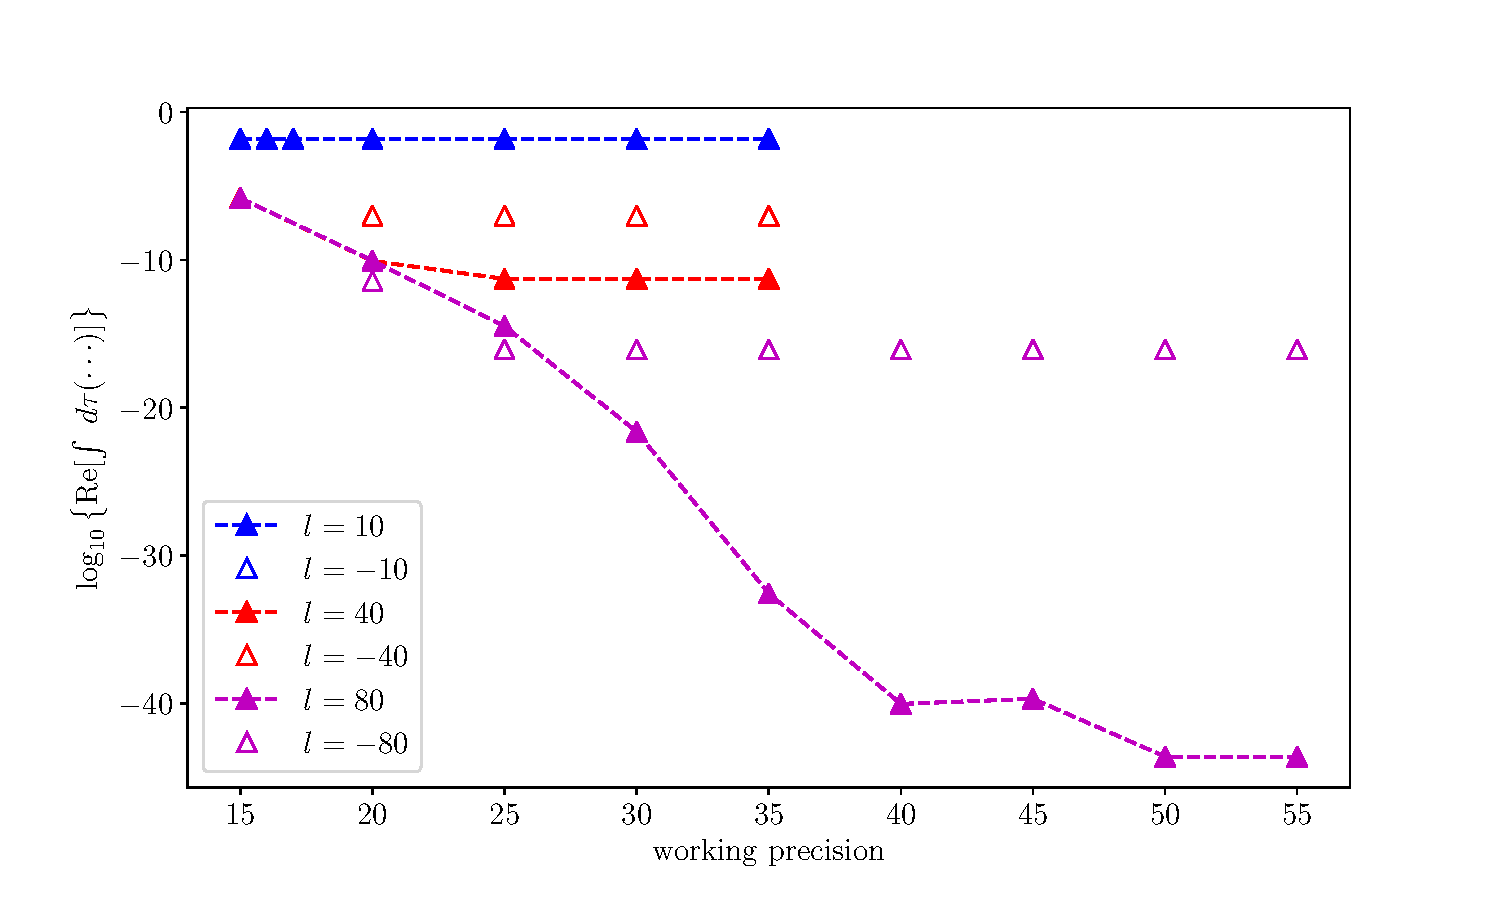
\includegraphics[width=0.75\textwidth]{figures/ch_ATI_SFA/He/n512PG25MR35l_pm104080logRe}
  \caption{Numerical evaluation of the time integral $F(l)$ contained
    in the transition amplitude~(\ref{eq:Mp_rew}) for $|l| = 10, 40,
    80$, indicated in blue, red and magenta respectively, as a
    function of the working precision requested.}
  \label{fig:WP_convergence}
\end{figure}


% include a figure of how the imaginary part converges to zero as the
% working precision is increased


Given that the transition amplitude that describes the rescattering of
an electron to its binding potential~(\ref{eq:Mp_quad}) is a
generalization of the Keldysh
amplitude~(\ref{eq:keldysh_amp_explicit}) one should expect that the
generalized ATI spectrum contains that of direct electrons at low
electron energies. A comparison between Eqs.~(\ref{eq:Mp_rew})
and~(\ref{eq:keldysh_amp_explicit}) illustrates that, for a given
value of $l$, the function $F(l)$ should be proportional to the Bessel
factor $J_{l}\left( \frac{U_{p}}{2\omega} \right)$. This calculation
was carried out for different values of $l$ in order to corroborate
the validity of the aforementioned generalization.

Figure~\ref{fig:integral_keldysh} exhibits a comparison of the
numerical evaluation of $F(l)$ in~(\ref{eq:Mp_rew}) with the simple
Bessel function in~(\ref{eq:keldysh_amp_explicit}) for several sets of
increasing values of $l_{\rm{max}}$. The coefficients that replace the
integral in the Keldysh amplitude were scaled, divided by a factor of
$5$, so it is possible to see the agreement. For negative values of
$l$, at about $l=-30$, the curves begin to differ as the integrals
oscillate around $10^{-6}\ \rm{(arb.\ units)}$ for a range of negative
$l$ values that extends from $l\approx -30$ to $l\approx -60$,
indicating the presence of rescattering as opposed to the case for the
direct transmission, shown as blue dots, from the Keldysh
amplitude. As one might notice, for sufficiently small negative values
of $l$ ($l < -60$) the values of the integral start dropping below,
indicating that convergence of the ionization spectrum for
rescattering electrons is to be expected. As the Bessel order, $l$,
was increased in the evaluation of the quadrature, the working
precision and precision goal were tuned appropriately so the curves
would remain comparable. This is consistent with
Figure~\ref{fig:WP_convergence}, as the order of Bessel functions
increases, a higher working precision is required in order to find a
numerical solution to the quadrature.

%As you can see the first 10 points (Lmin=-80 to -70) are smaller
%compared to the others, so convergence can be expected.

\begin{figure}
\begin{subfigure}[b]{0.33\linewidth}
  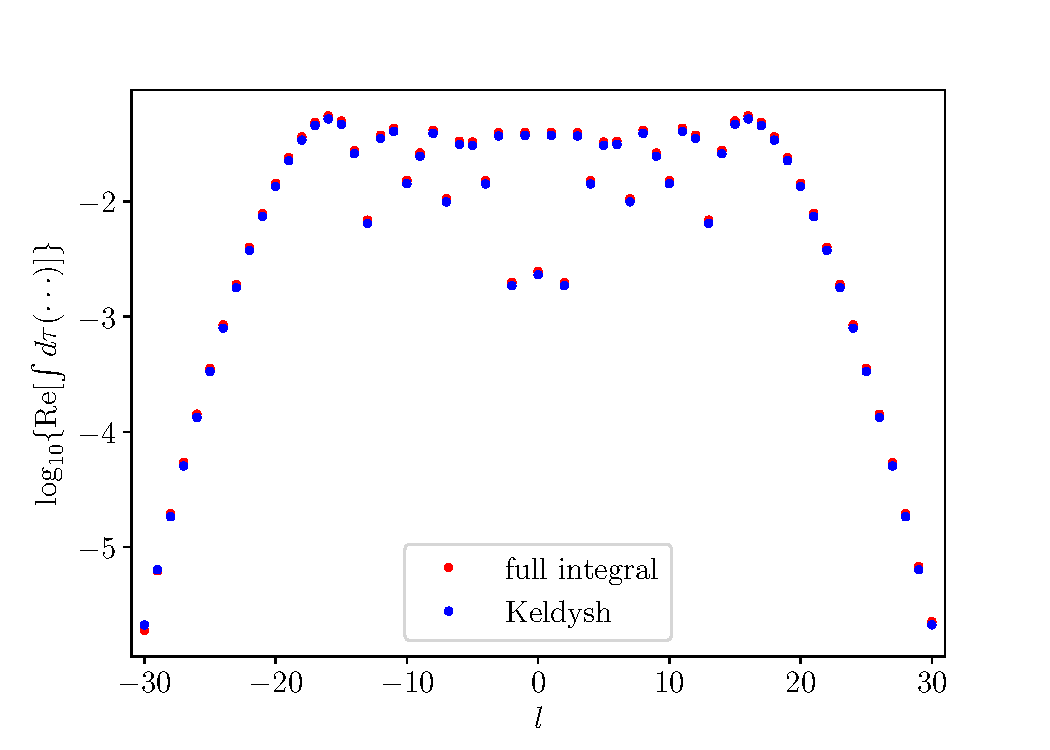
\includegraphics[width=\textwidth]{figures/ch_ATI_SFA/He/l30n512WP20PG15MR35vsKeldysh.pdf}
\end{subfigure}
\begin{subfigure}[b]{0.33\linewidth}
  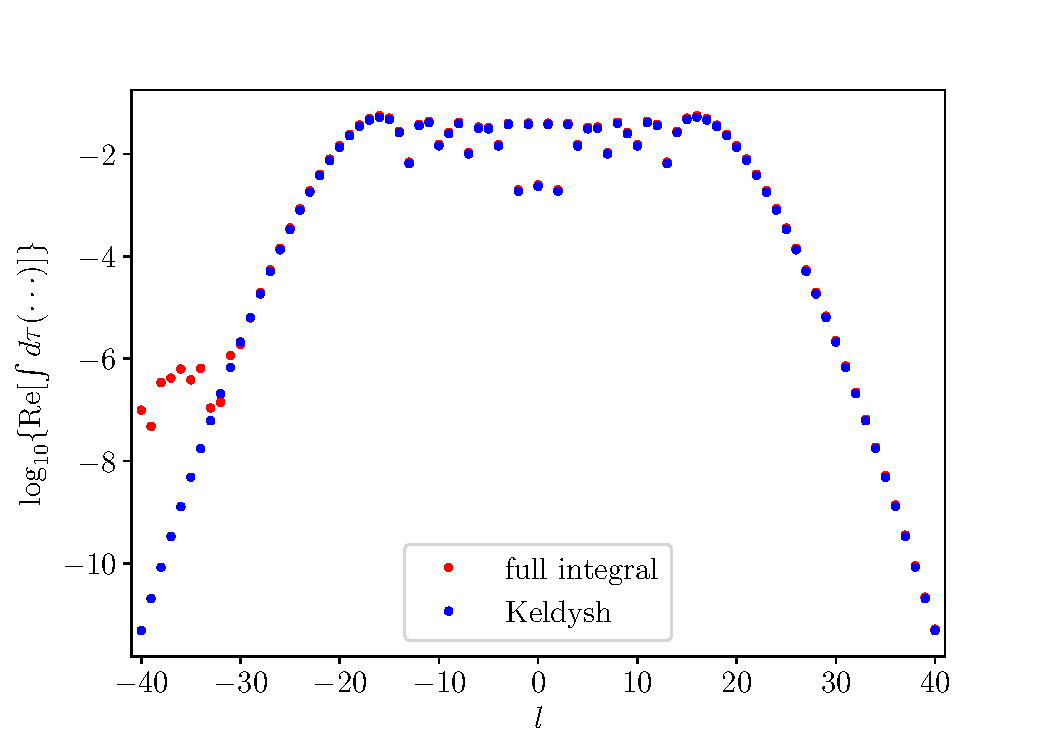
\includegraphics[width=\textwidth]{figures/ch_ATI_SFA/He/l40n512WP40PG25MR35vsKeldysh.pdf}
\end{subfigure}
\begin{subfigure}[b]{0.33\linewidth}
  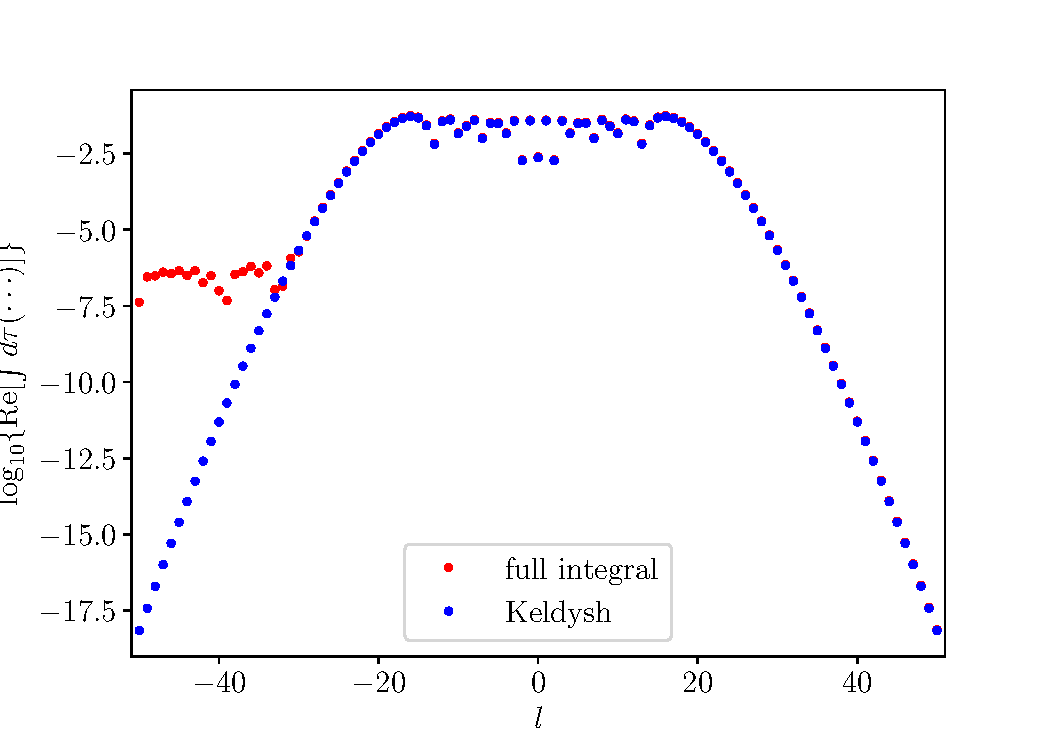
\includegraphics[width=\textwidth]{figures/ch_ATI_SFA/He/l50n512WP40PG25MR35vsKeldysh.pdf}
\end{subfigure}
\begin{subfigure}[b]{0.33\linewidth}
  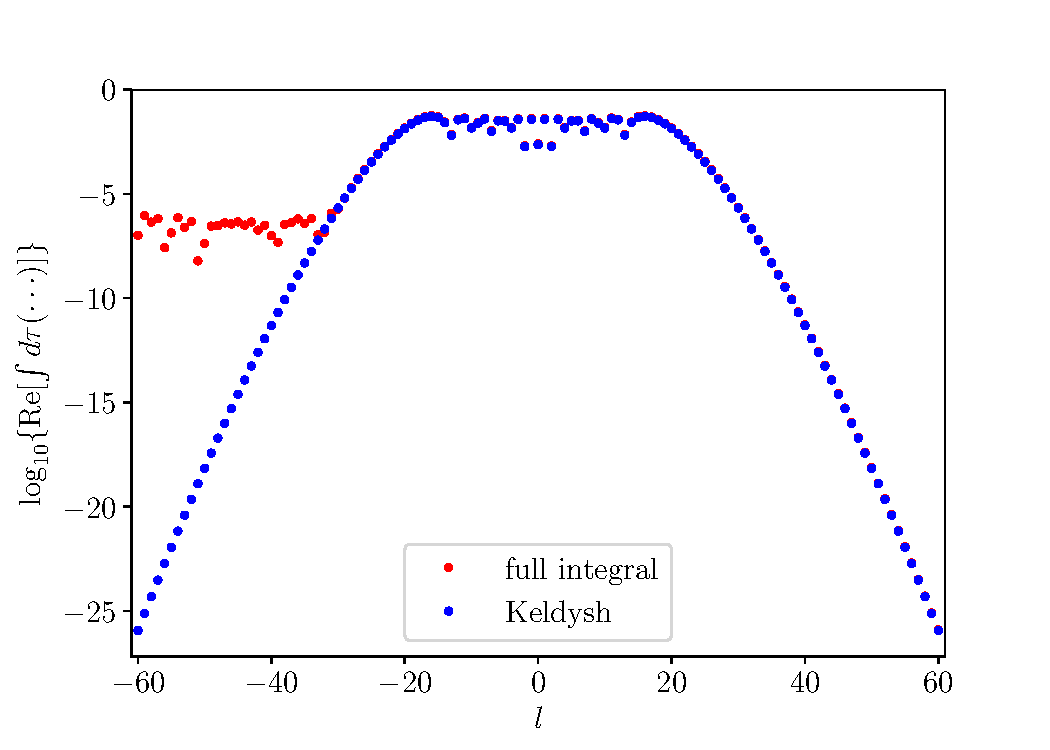
\includegraphics[width=\textwidth]{figures/ch_ATI_SFA/He/l60n512WP40PG25MR35vsKeldysh.pdf}
\end{subfigure}
\begin{subfigure}[b]{0.33\linewidth}
  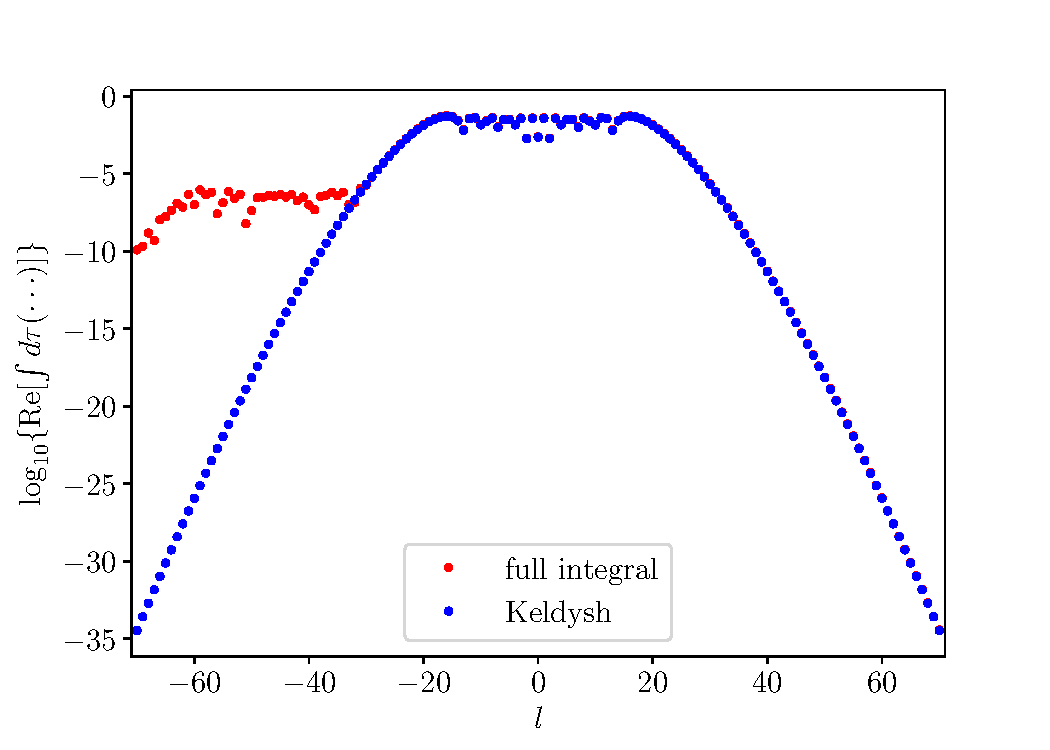
\includegraphics[width=\textwidth]{figures/ch_ATI_SFA/He/l70n512WP40PG25MR35vsKeldysh.pdf}
\end{subfigure}
\begin{subfigure}[b]{0.33\linewidth}
  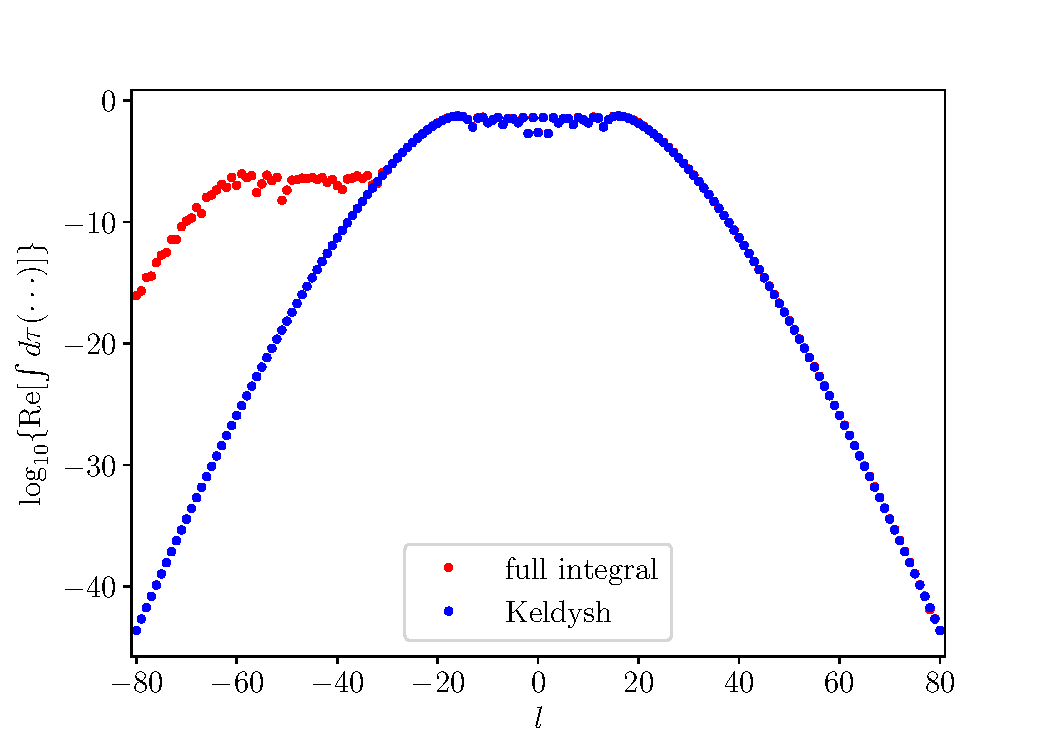
\includegraphics[width=\textwidth]{figures/ch_ATI_SFA/He/l80n512WP50PG25MR35vsKeldysh.pdf}
\end{subfigure}
\caption{Numerical evaluation of the time integral $F(l)$ contained in
  the transition amplitude~(\ref{eq:Mp_rew}) (red dots) in contrast
  with its analogous Bessel term in the Keldysh amplitude for direct
  transmission (blue dots) for zero-range He atom model as a function
  of the Bessel function order $l$ for increasing values of
  $l_{\rm{max}}$, $l=[ -l_{\rm{max}} , \dots, l_{\rm{max}}]$.}
  \label{fig:integral_keldysh}
\end{figure}

% include convergence of the spectrum that yields from keldysh
% amplitude for direct electrons

% include convergence of ATI spectrum including rescattering with
% remark that it contains the spectrum of direct electrons for low p_x

The ionization spectrum for the He model for emission parallel to the
electric field of the laser that contains the contribution of direct
electrons, given by the Keldysh
amplitude~(\ref{eq:keldysh_amp_explicit}), is shown in
Figure~\ref{fig:keldysh_convergence}. For a given electron energy, the
sum over the Bessel order was extended up to increasing values of
$l_{\rm{max}}$, ranging from $20$ to $50$, in order to display the
convergence of the spectrum in the limit $l\to\infty$. For
$l_{\rm{max}}$ values as low as $20$ and $30$ the final structure of
the spectrum for very small energies, $<1 \rm{U_{p}}$, begins to be
visible. However, more terms need to be considered in the sum over
Bessel functions in order to obtain the converged spectrum. The yield
consisting only of direct electrons converges relatively fast to its
final shape (dash-dotted line) in which a sequence of narrow
suppressions of the probability amplitude separated by rounded tops
drops as the electron energy increases and eventually vanishes at
about $2.5\rm{U_{p}}$.

\begin{figure}
  \centering
  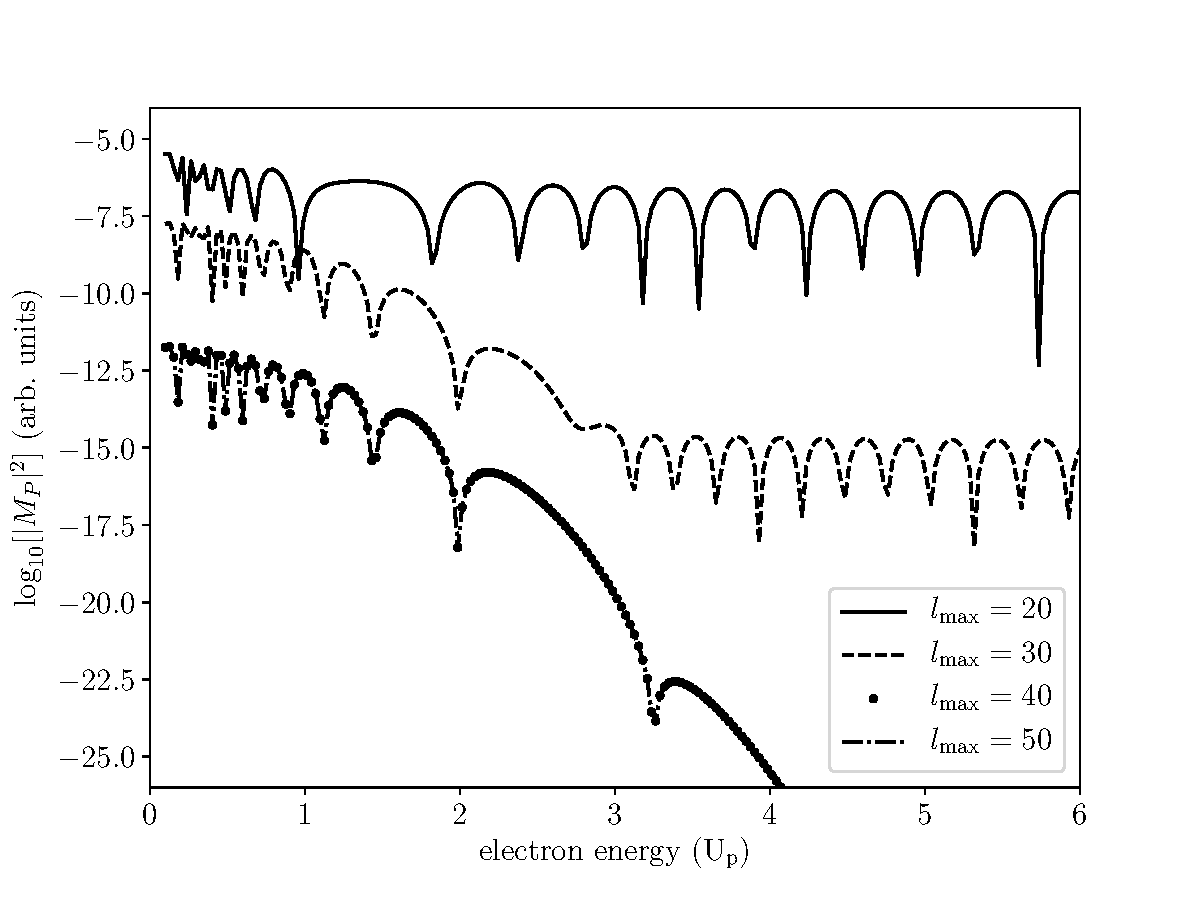
\includegraphics[width=0.75\textwidth]{figures/ch_ATI_SFA/He/l20304050Keldysh.pdf}
\caption{ATI spectrum of zero-range model for helium by a linearly
  polarized field with a laser intensity of $10^{15}\ \rm{W/cm^{2}}$
  with $\hbar\omega = 1.58\ \rm{eV}$ describing direct electrons. Each
  curve corresponds to a finite value of $l_{\rm{max}}$ in the
  standard Keldysh amplitude.}
\label{fig:keldysh_convergence}
\end{figure}

The results of the calculations based on~(\ref{eq:Mp_quad}) are shown
in Figure~\ref{fig:mp_convergence}. Each coloured curve represents the
ionization amplitude for an atom of He under a strong-laser field for
increasing values of the Bessel function order, $l$. As one might
notice, the ionization spectrum converges for $l=80$ (bottom right
plot) after undergoing some fluctuations for $l$ values between $40$
and $70$. The spectrum for direct electrons (black dots) is included
as a reference. As it can be seen, both the standard Keldysh amplitude
and the fully quantum mechanical result that incorporates rescattering
exhibit very similar electron yields for energies lower than
$2.5\rm{U_{p}}$ where the spectrum is consisting only of direct
electrons. As the electron energy increases, the rescattered electrons
begin to exceed the direct ones and the curves start to differ from
each other. The transition probability, consisting almost exclusively
of rescattered electrons, reaches a plateau consisting of a sequence
of suppressions separated by rounded tops. This behaviour is a direct
consequence of quantum interference, as the released electrons
interfere constructively and destructively in every optical cycle of
the laser field as a function of energy. For large energies of about
$10\rm{U_{p}}$ the plateau shows a cutoff that indicates the end of
the rescattering spectrum. The position of this cutoff as well as the
onset energy of the plateau fluctuate with the orientation of the
emitted electrons with respect to the electric field of the laser as
well as with variations of the intensity of the
field~\cite{Kopold_1997sfa,Paulus_1994plateau,Paulus_1994plateau_classical}.


\begin{figure}
\begin{subfigure}[b]{0.5\linewidth}
  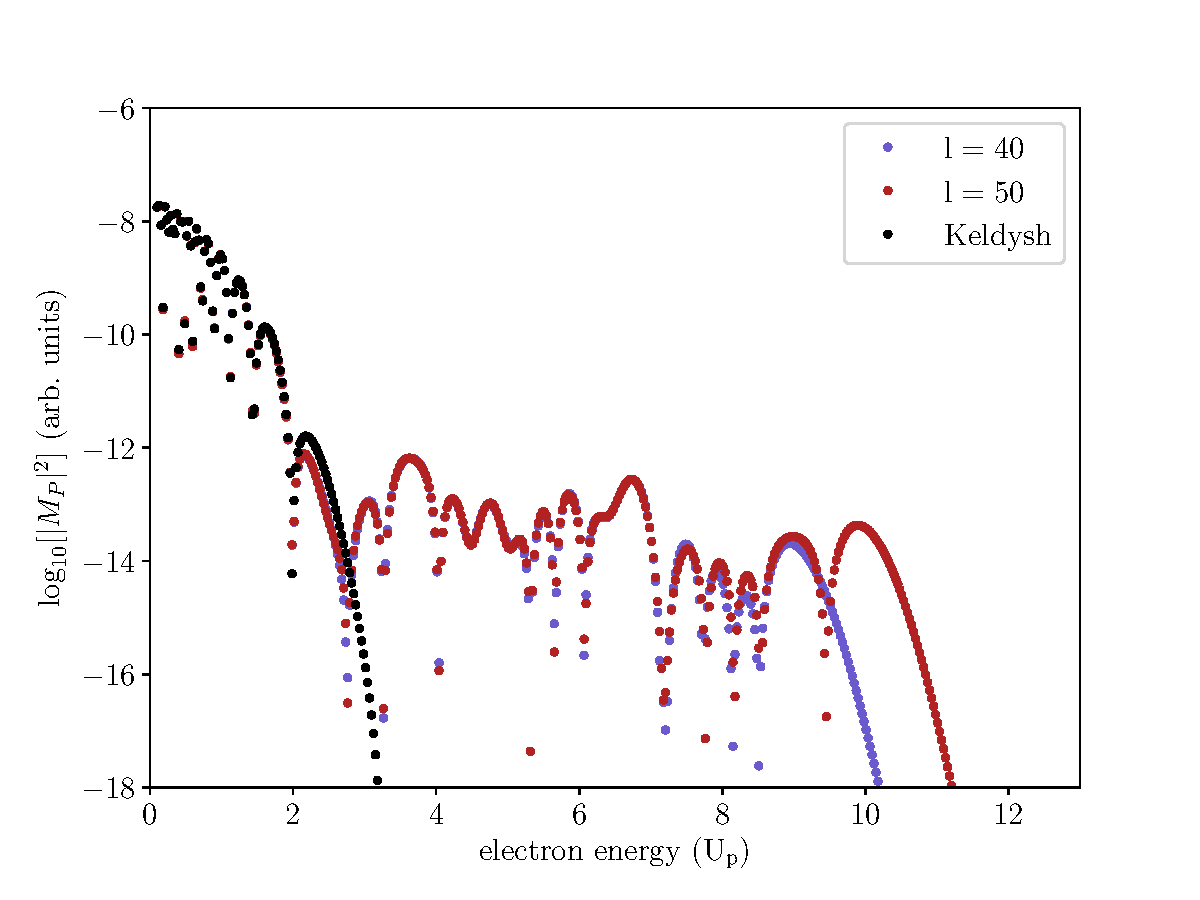
\includegraphics[width=\textwidth]{figures/ch_ATI_SFA/He/l4050n512WP40PG25MR35vsKeldysh.pdf}
\end{subfigure}
\begin{subfigure}[b]{0.5\linewidth}
  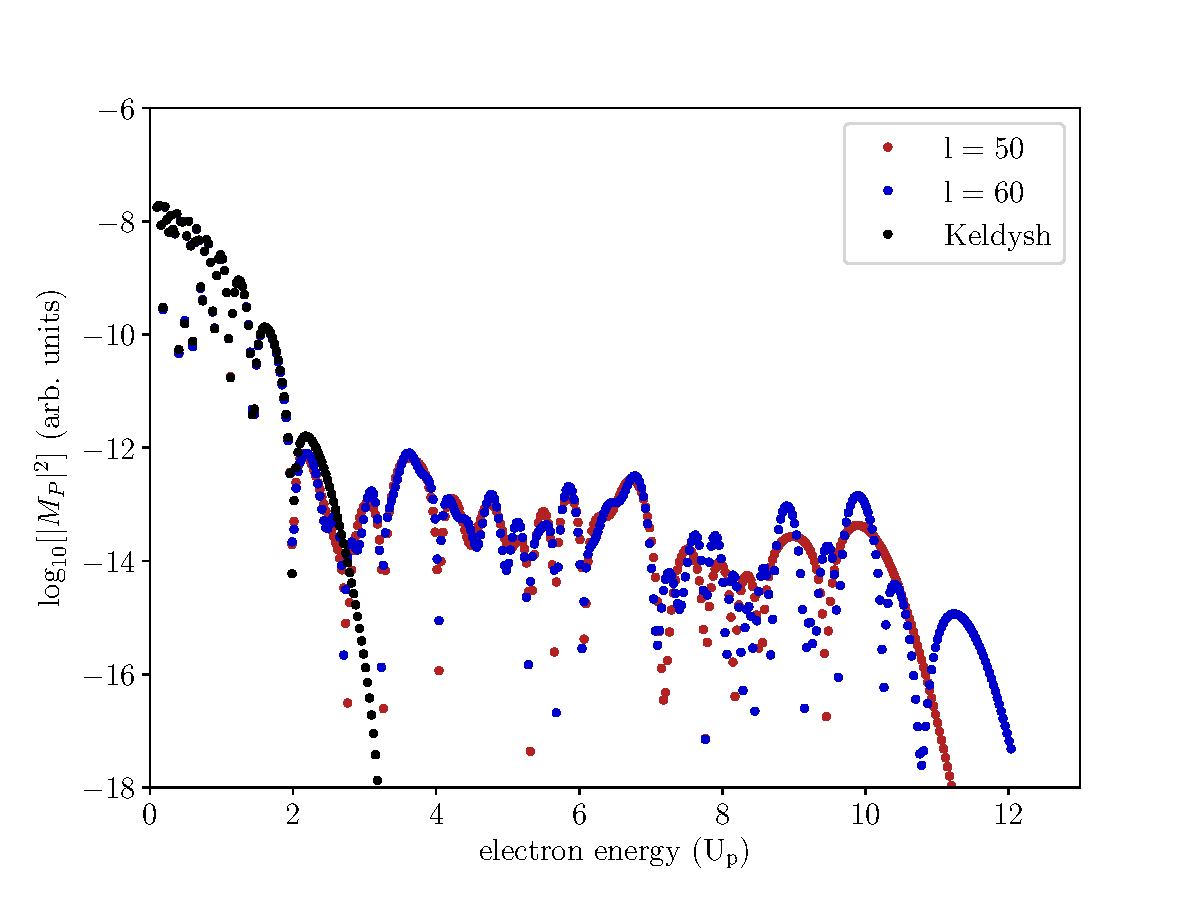
\includegraphics[width=\textwidth]{figures/ch_ATI_SFA/He/l5060n512WP40PG25MR35vsKeldysh.pdf}
\end{subfigure}
\begin{subfigure}[b]{0.5\linewidth}
  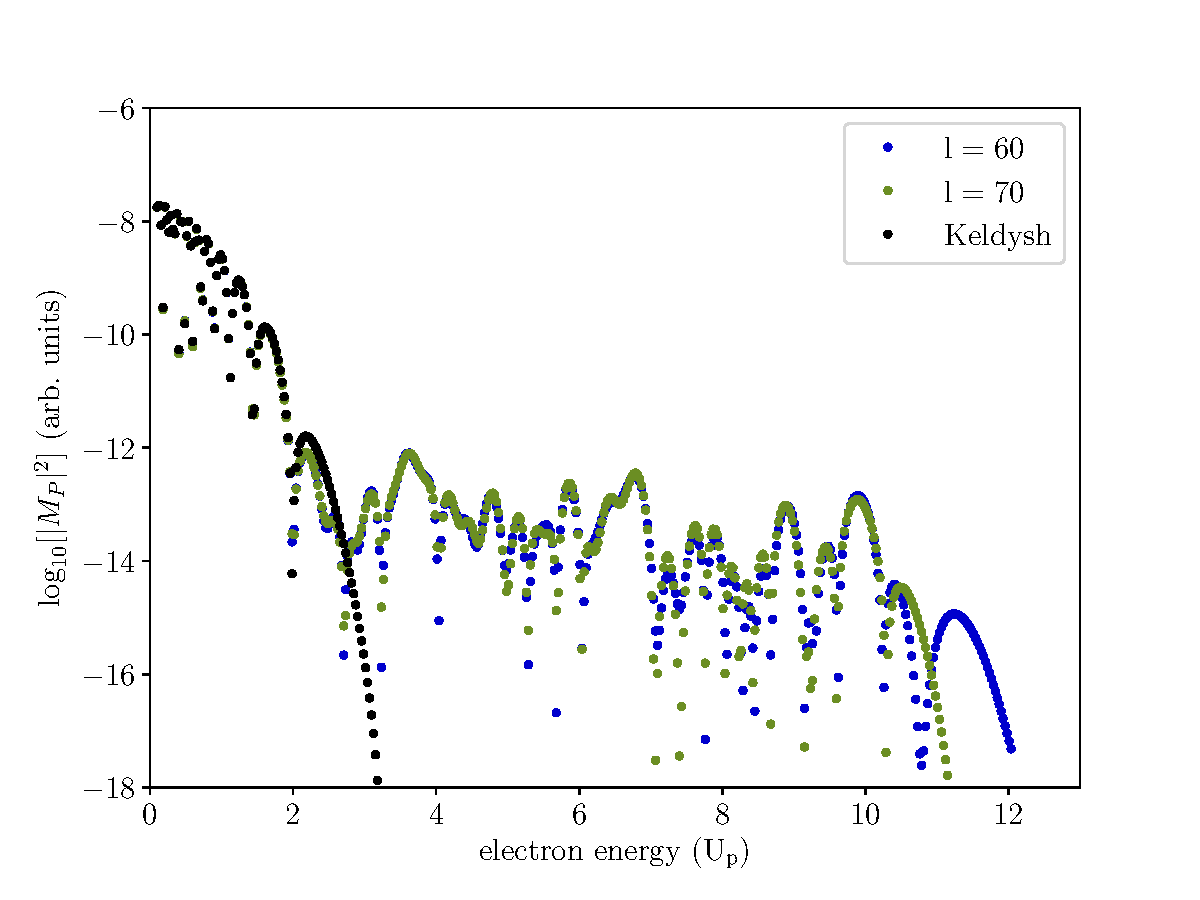
\includegraphics[width=\textwidth]{figures/ch_ATI_SFA/He/l6070n512WP40PG25MR35vsKeldysh.pdf}
\end{subfigure}
\begin{subfigure}[b]{0.5\linewidth}
  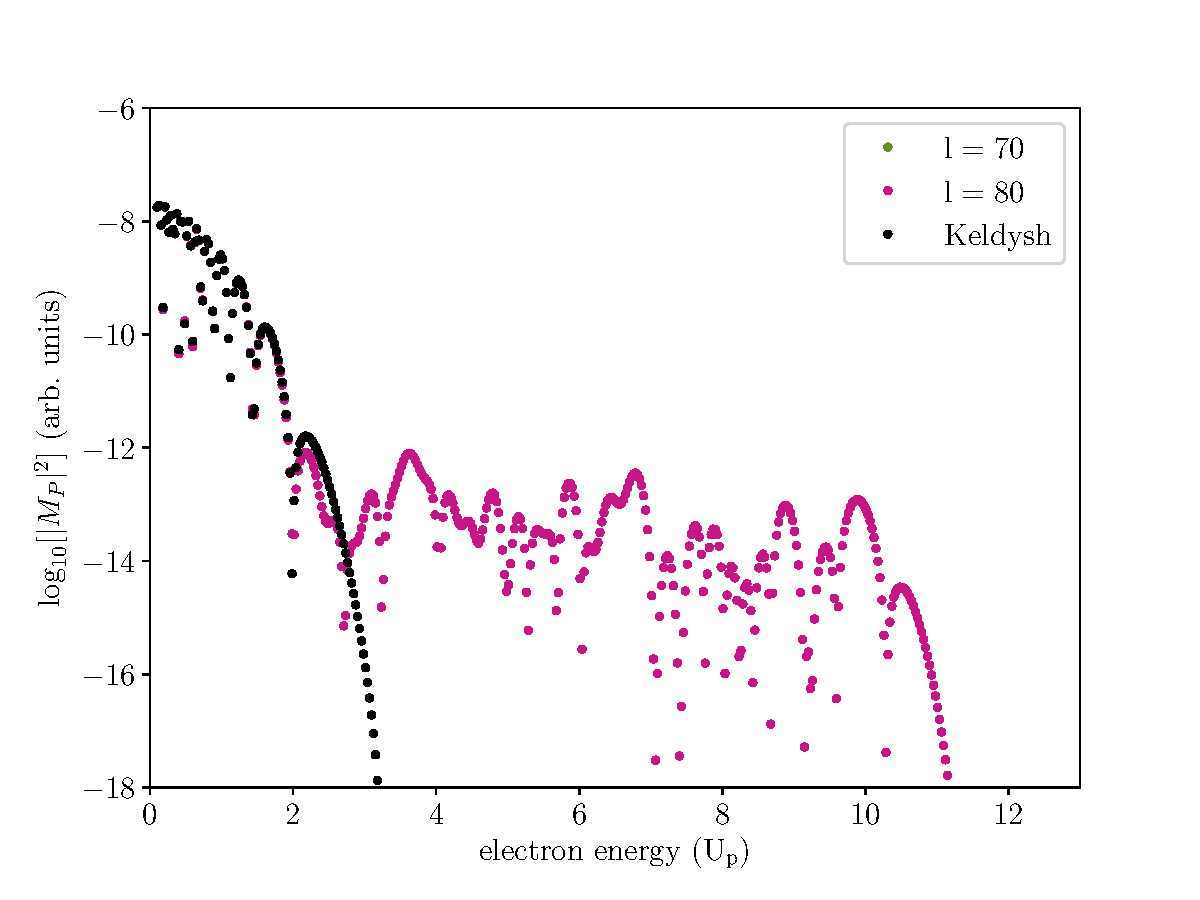
\includegraphics[width=\textwidth]{figures/ch_ATI_SFA/He/l7080n512WP40PG25MR35vsKeldysh.pdf}
\end{subfigure}
\caption{ATI spectrum of a zero-range He model with a binding energy
  of $E_{0} = -0.9\ \rm{a.u.}$ by a linearly polarized field with a
  laser intensity of $10^{15}\ \rm{W/cm^{2}}$ with $\hbar\omega =
  1.58\ \rm{eV}$ in terms of an increasing Bessel order,
  $l_{\rm{max}}$, as a function of the electron energy (in
  colour). The result from the standard Keldysh approximation is shown
  as the black dotted line.}
  \label{fig:mp_convergence}
\end{figure}


\subsection{\label{sec:mo_sfa} Ionization spectrum for the $1b_{1}$ and $1b_{2}$ orbitals
  of H$_{2}$O}
% eq.9 and 11 for 1b1 and 1b2 MOs

% mention studies of the h2o molecule under a laser field, put it in
% terms of wanting to explore the molecular orbital response


% mention that 1b1 and 1b2 MOs were modelled previously as spherical
% orbitals, where only a radial dependence was included in the
% effective potential, under this approximation we extended our study
% to model how this approximate orbitals would ionize in the presence
% of a strong laser field
The study on the H$_{2}$O molecular orbitals presented in
Chapter~\ref{cha:dc_h2o} is extended in this section with the aim of
exploring the ATI spectrum of the $1b_{1}$ and $1b_{2}$ molecular
orbitals previously characterized as spherical orbitals. The
zero-range model calculation carried out in the previous section
combined with the strong-field approximation is applied to these
valence orbitals in order to explore their response to an intense
laser field.

%With the aim of exploring the ionization regime of the water molecule
%in terms of the molecular orbital response to an intense laser field,
%the zero-range model calculation discussed in the previous section, in
%which the binding potential of the atom is considered to act on the
%scattered electrons as a delta function, is applied to the H$_{2}$O
%valence orbitals $1b_{1}$ and $1b_{2}$.

% mention more the details of the calculation
Each molecular orbital is treated as an independent atom in which the
eigenvalues $\epsilon_{1b_{1}}$ and $\epsilon_{1b_{2}}$ obtained from
the radial representation of their effective potentials,
$V_{\rm{eff}}(r)$, are considered their binding energies,
respectively. With this in mind, it is possible to generate the
ionization spectrum for direct electrons and that for rescattering
electrons that would correspond to each molecular orbital under a
strong-laser field. Inserting the molecular binding energies into
Eqs.~(\ref{eq:keldysh_amp_explicit}) and~(\ref{eq:Mp_quad}) one can
explore the convergence of the ionization spectrum in terms of the
number of Bessel functions included in their respective sums.

% describe the plots comparing direct and rescattering electrons
% describe convergence of the spectrum
Similarly to the case of strong-field ionization of a zero-range He
model, the quadrature $F(l)$ in~(\ref{eq:Mp_rew}) remains to be solved
in order to obtain the ionization spectrum for rescattered
electrons. The general expression~(\ref{eq:Mp_quad}), which encloses
the limiting case of ionization of direct electrons, generates an
electron yield which follows that of direct electrons for low
energies, i.e., electrons energies for which the direct spectrum is
not vanished and the rescattering effects are not taken into
account. This section is aimed to validate the previous statement and
explore the convergence of the ATI spectrum of these two simplified
representations of H$_{2}$O orbitals.

Figures~\ref{fig:1b1_vs_keldysh} and~\ref{fig:1b2_vs_keldysh} show the
values taken by the function $F(l)$ for a set of values of
$l_{\rm{max}}$, $l_{\rm{max}} = 30,\dots,80$, that indicate the
extension of the sum~(\ref{eq:Mp_quad}) in terms of Bessel functions
and the Bessel term in the standard Keldysh
amplitude~(\ref{eq:keldysh_amp_explicit}) in red and blue,
respectively. The numerical values of the integral $F(l)$ were
rescaled for both molecular orbitals, divided by a factor of $5.5$ for
the $1b_{1}$ MO and by a factor of $6.5$ for the $1b_{2}$ MO, in order
to make the comparability between the curves visible. Correspondingly,
the working precision of the calculations was gradually increased for
$|l| > 0$ up to a maximum of $50$ digits of precision for
$l_{\rm{max}} = 80$. As it has been observed for ionization along the
electric field of the laser for a He atom~\cite{Kopold_1997sfa}, the
precise agreement between the emission rate for direct electrons and
the full ionization spectrum including rescattering for energies below
the cutoff of the direct-electron spectrum indicates that a
correlation between the red and blue curves should be expected for a
range of values of $l_{\rm{max}}$ before deviations due to
rescattering become substantial. This behaviour can be observed for
both molecular orbitals for $l < -30$, where the quadrature $F(l)$
reaches a plateau at about $10^{-5}$ that extends up to about $l <
-60$ where signs of convergence of the time integral $F(l)$ become
noticeable as the red curve begins to decline.

\begin{figure}
  \begin{subfigure}[b]{0.33\linewidth}
    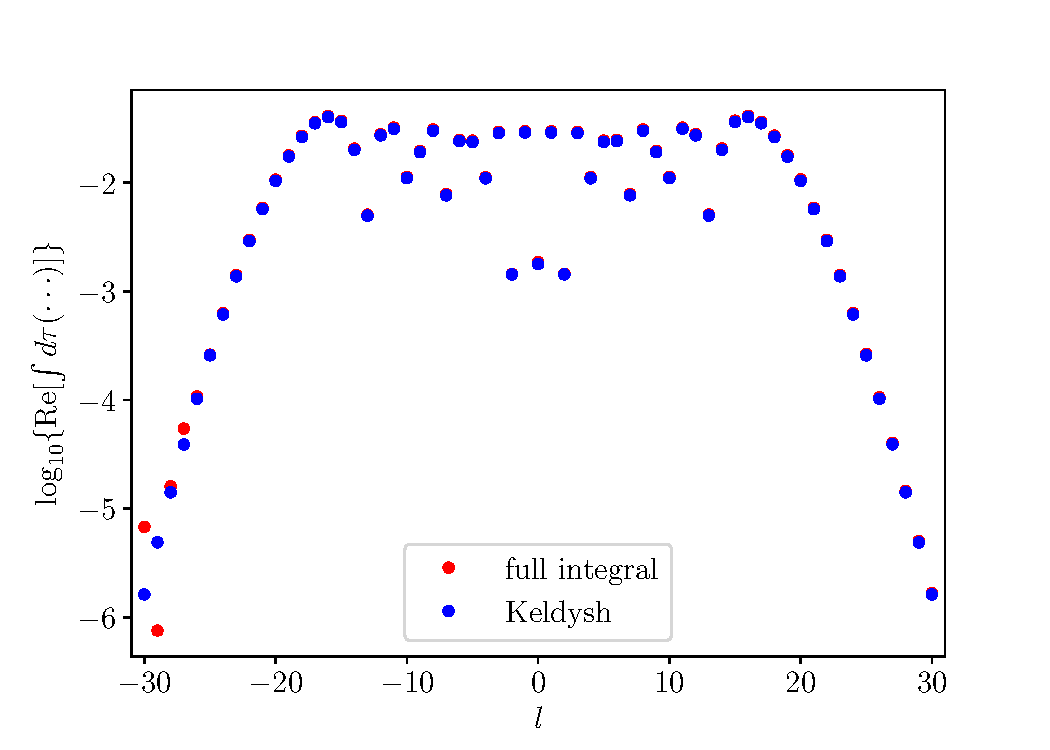
\includegraphics[width=\textwidth]{figures/ch_ATI_SFA/1b1/l30n512WP20PG15MR35vsKeldysh.pdf}
  \end{subfigure}
  \begin{subfigure}[b]{0.33\linewidth}
    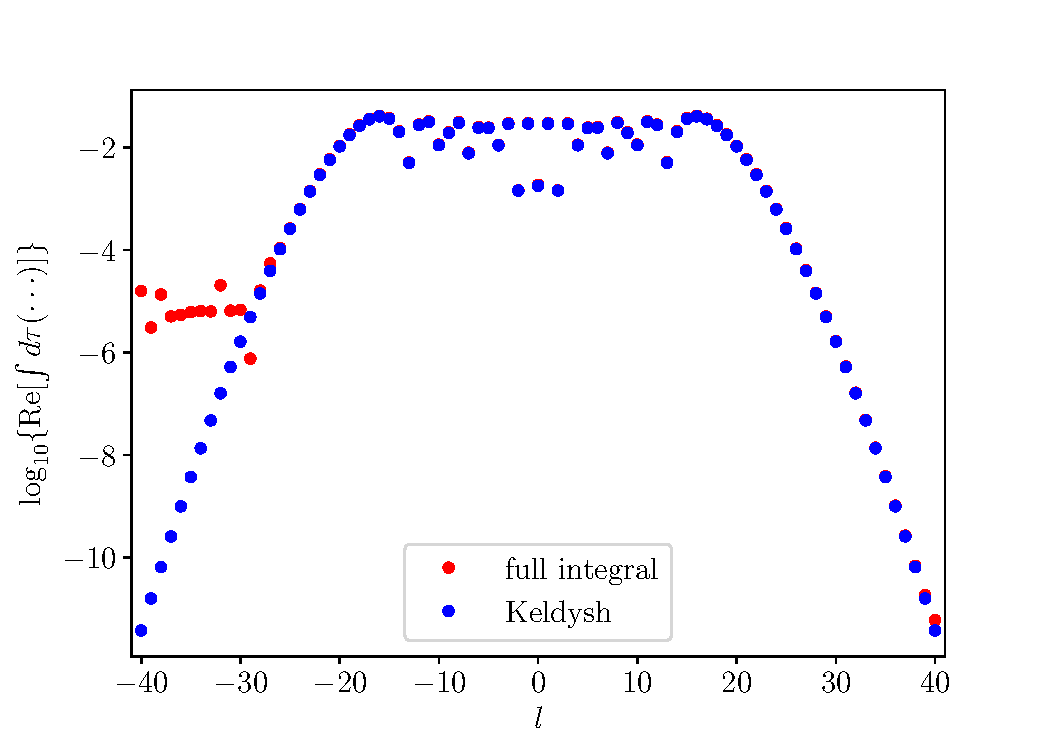
\includegraphics[width=\textwidth]{figures/ch_ATI_SFA/1b1/l40n512WP20PG15MR35vsKeldysh.pdf}
  \end{subfigure}
  \begin{subfigure}[b]{0.33\linewidth}
    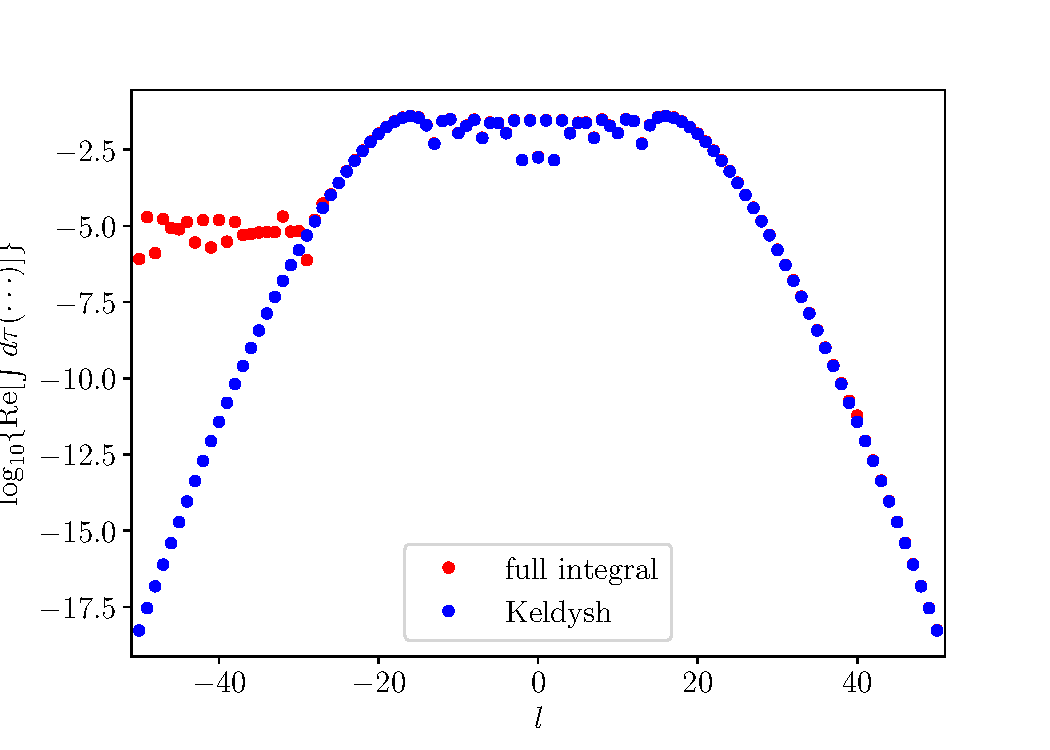
\includegraphics[width=\textwidth]{figures/ch_ATI_SFA/1b1/l50n512WP40PG25MR35vsKeldysh.pdf}
  \end{subfigure}
  \begin{subfigure}[b]{0.33\linewidth}
    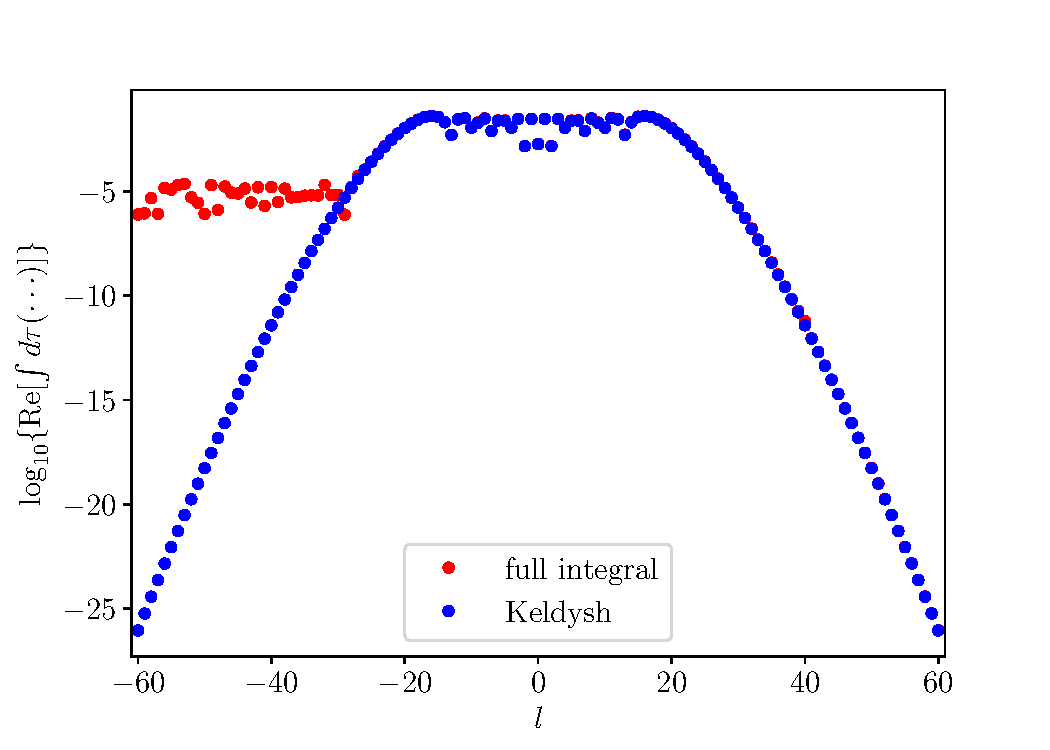
\includegraphics[width=\textwidth]{figures/ch_ATI_SFA/1b1/l60n512WP40PG25MR35vsKeldysh.pdf}
  \end{subfigure}
  \begin{subfigure}[b]{0.33\linewidth}
    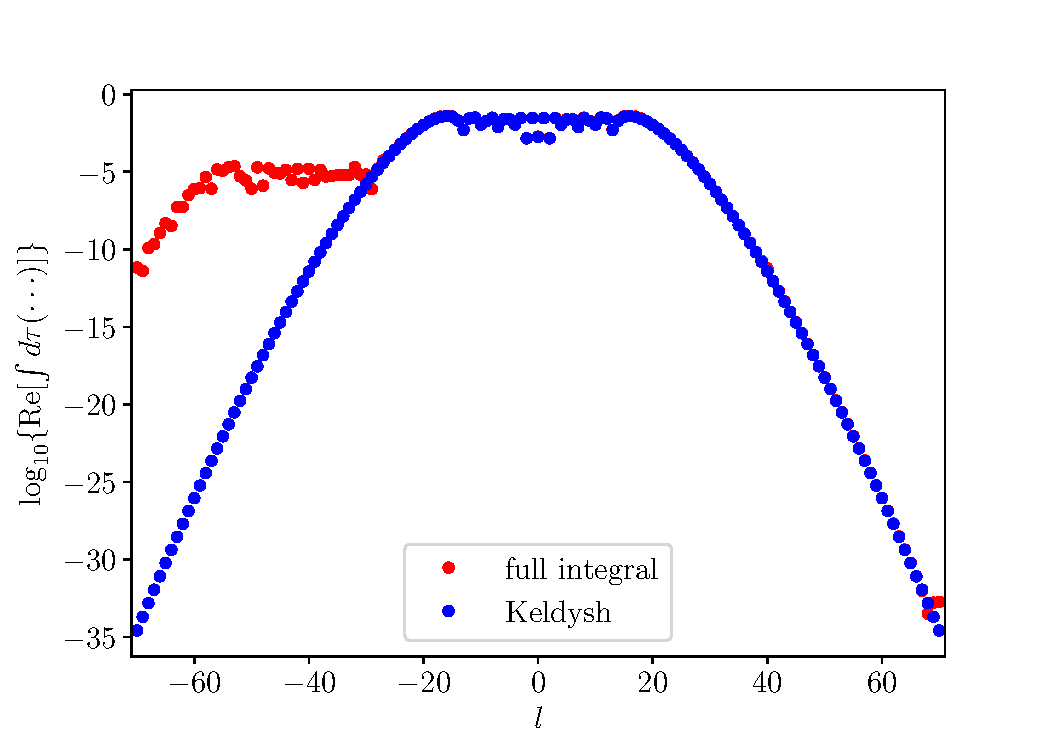
\includegraphics[width=\textwidth]{figures/ch_ATI_SFA/1b1/l70n512WP40PG25MR35vsKeldysh.pdf}
  \end{subfigure}
  \begin{subfigure}[b]{0.33\linewidth}
    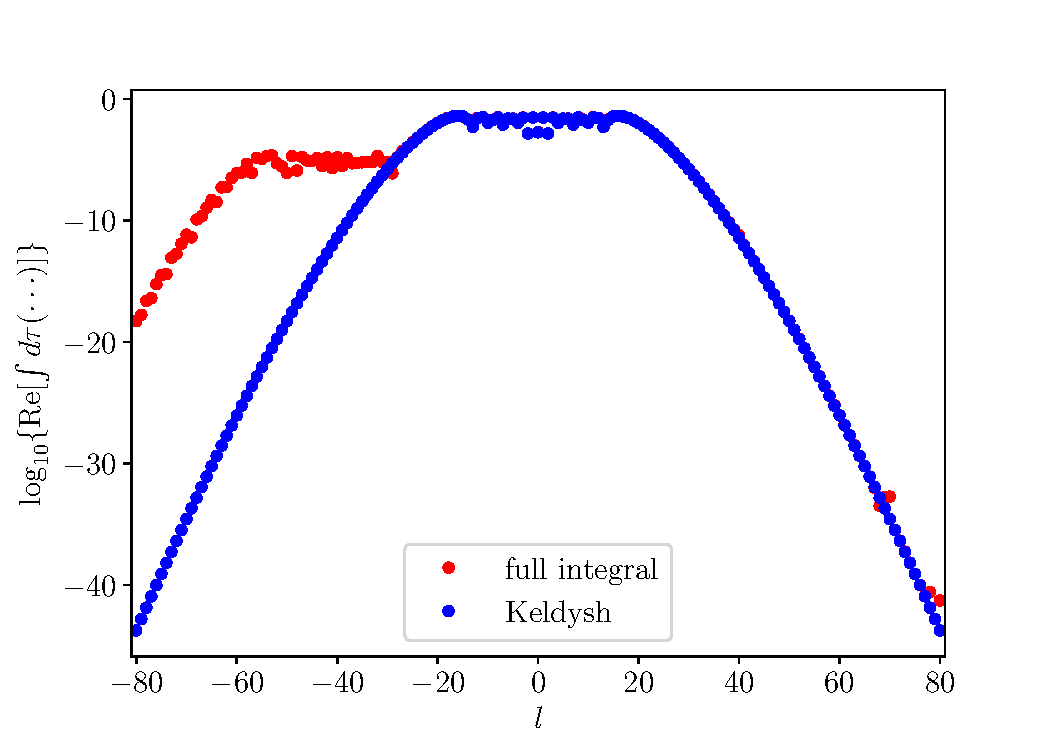
\includegraphics[width=\textwidth]{figures/ch_ATI_SFA/1b1/l80n512WP50PG25MR35vsKeldysh.pdf}
  \end{subfigure}
  \caption{Numerical evaluation of the time integral $F(l)$ in the
    transition amplitude~(\ref{eq:Mp_rew}) (red dots) in contrast with
    its analogous Bessel term in the Keldysh amplitude for direct
    transmission (blue dots) for the $1b_{1}$ MO of H$_{2}$O as a
    function of the Bessel function order $l$ for increasing values of
    $l_{\rm{max}}$, $l=[ -l_{\rm{max}} , \dots, l_{\rm{max}}]$.}
    \label{fig:1b1_vs_keldysh}
\end{figure}

\begin{figure}
  \begin{subfigure}[b]{0.33\linewidth}
    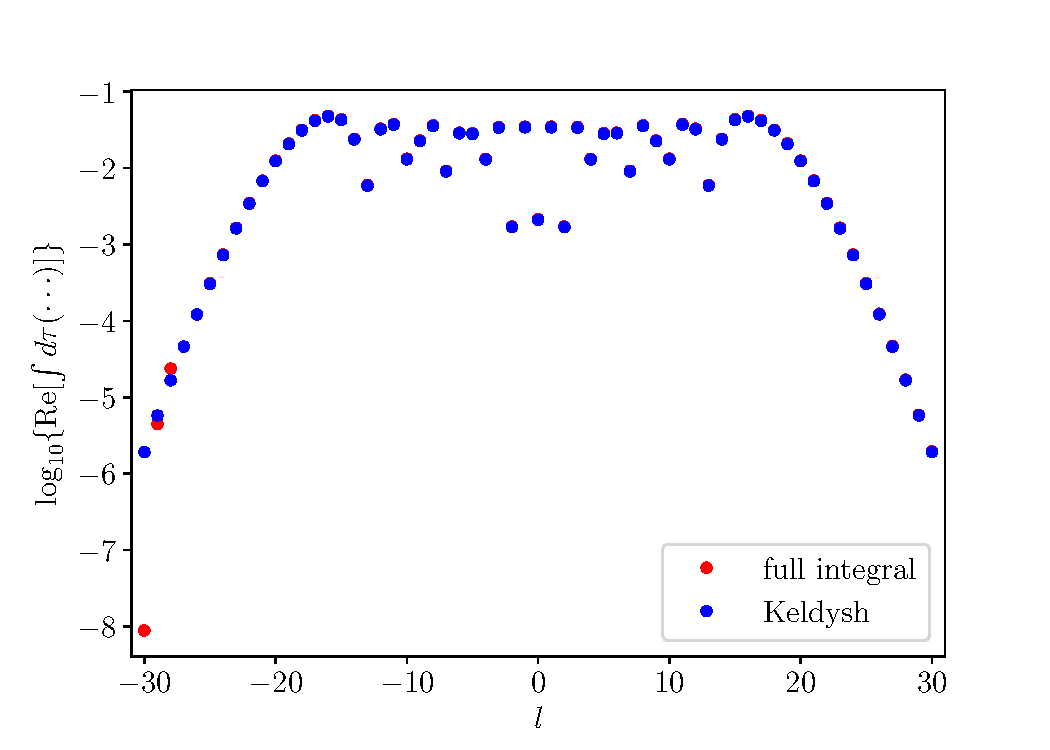
\includegraphics[width=\textwidth]{figures/ch_ATI_SFA/1b2/l30n512WP20PG15MR35vsKeldysh.pdf}
  \end{subfigure}
  \begin{subfigure}[b]{0.33\linewidth}
    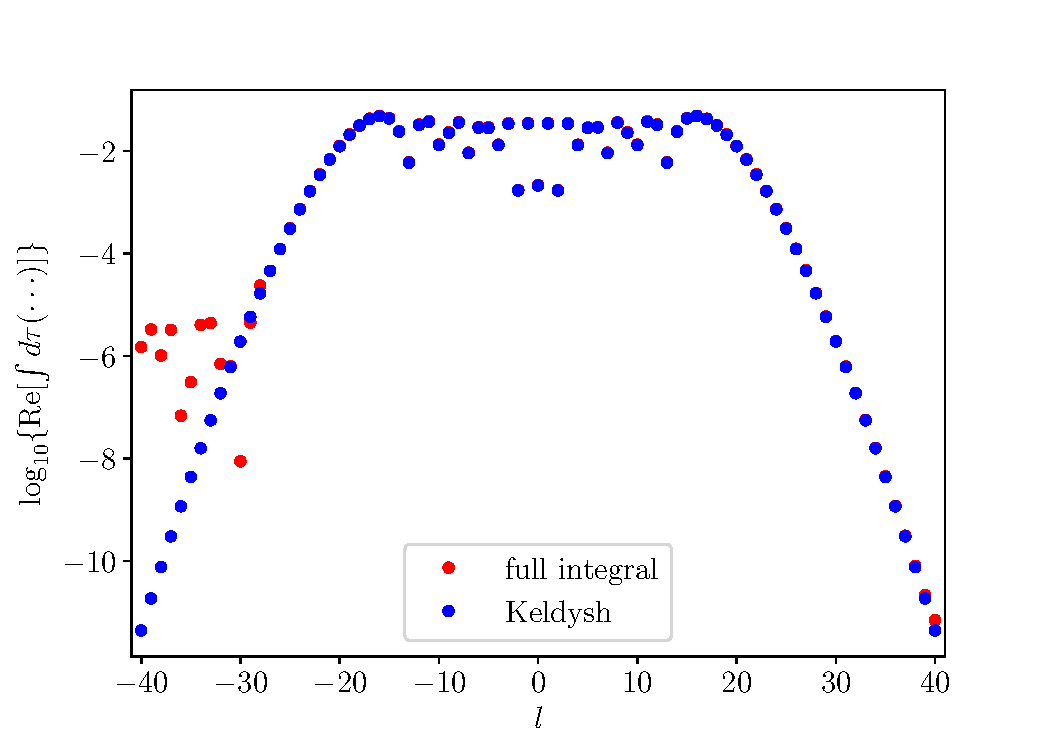
\includegraphics[width=\textwidth]{figures/ch_ATI_SFA/1b2/l40n512WP20PG15MR35vsKeldysh.pdf}
  \end{subfigure}
  \begin{subfigure}[b]{0.33\linewidth}
    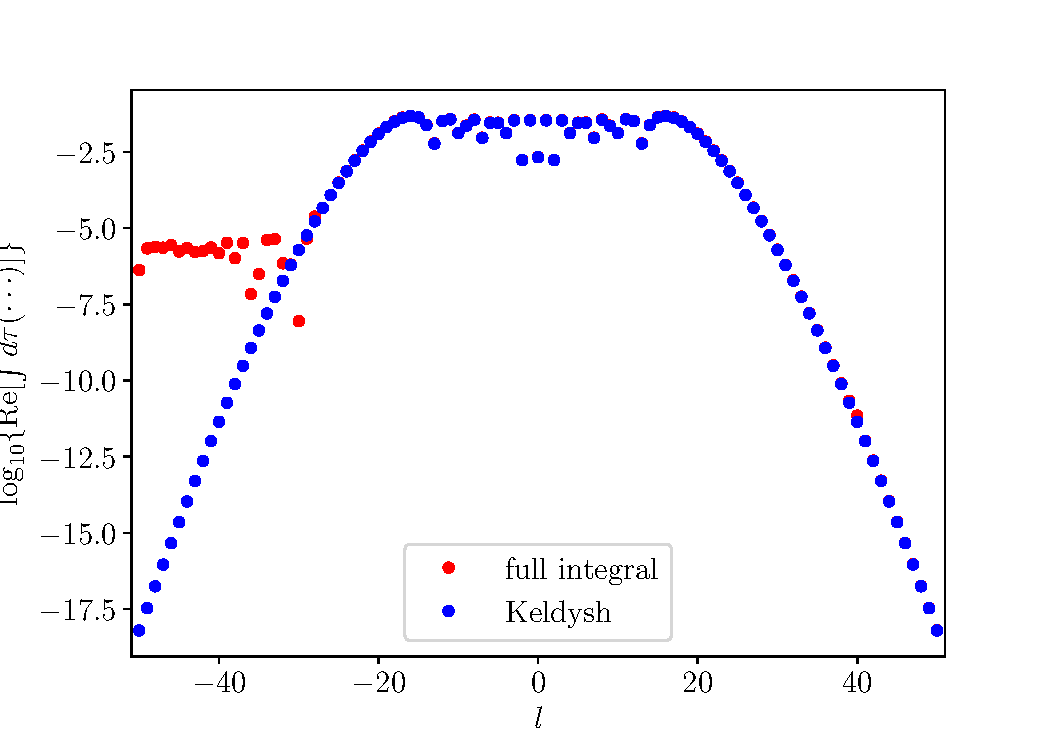
\includegraphics[width=\textwidth]{figures/ch_ATI_SFA/1b2/l50n512WP40PG25MR35vsKeldysh.pdf}
  \end{subfigure}
  \begin{subfigure}[b]{0.33\linewidth}
    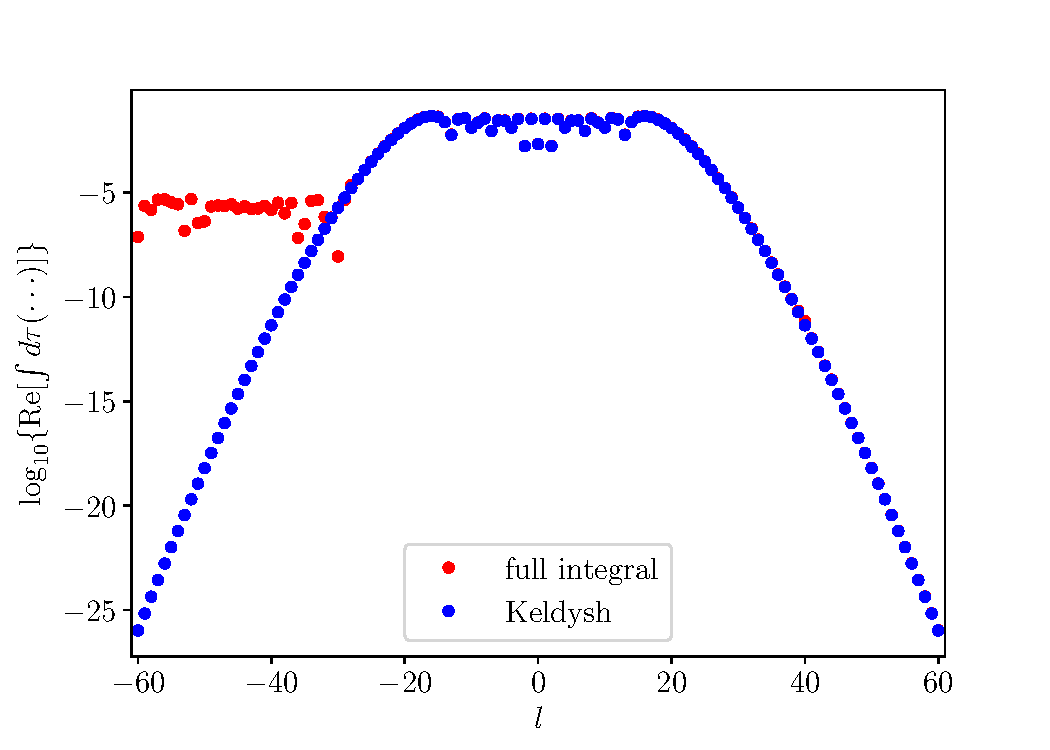
\includegraphics[width=\textwidth]{figures/ch_ATI_SFA/1b2/l60n512WP40PG25MR35vsKeldysh.pdf}
  \end{subfigure}
  \begin{subfigure}[b]{0.33\linewidth}
    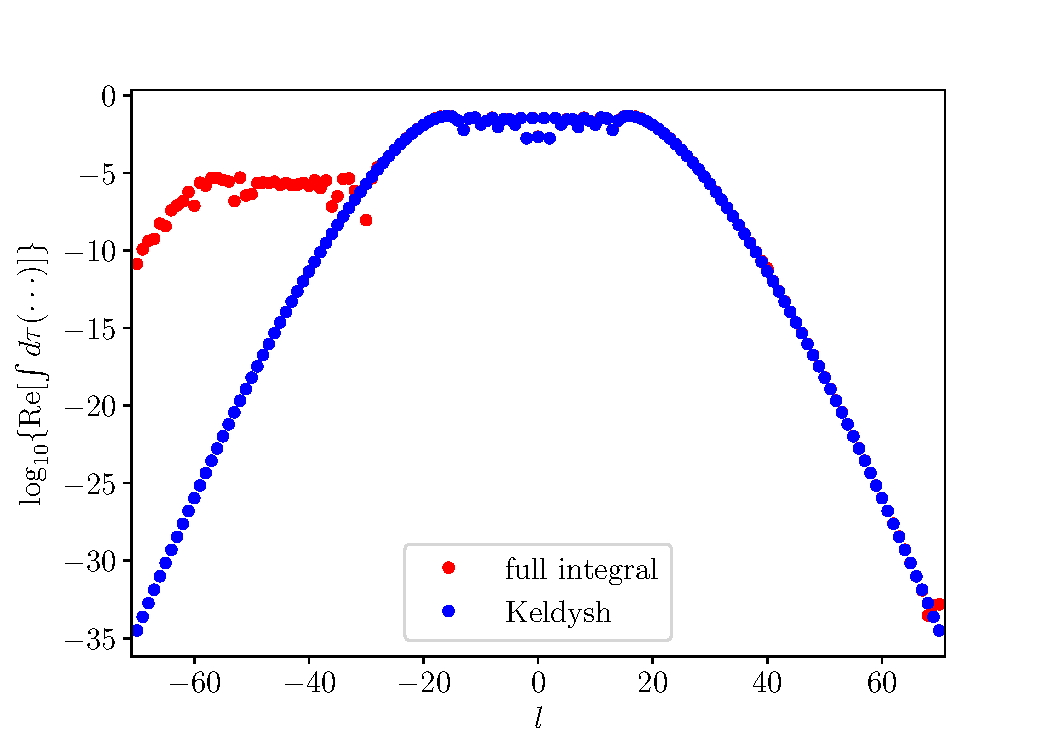
\includegraphics[width=\textwidth]{figures/ch_ATI_SFA/1b2/l70n512WP40PG25MR35vsKeldysh.pdf}
  \end{subfigure}
  \begin{subfigure}[b]{0.33\linewidth}
    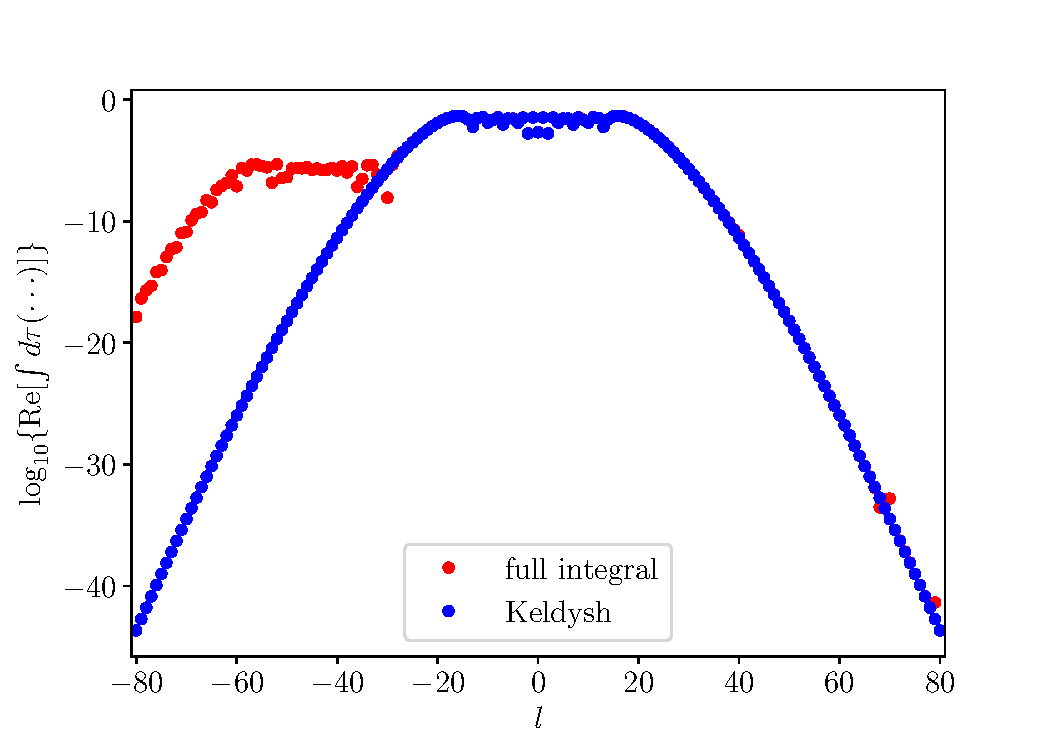
\includegraphics[width=\textwidth]{figures/ch_ATI_SFA/1b2/l80n512WP50PG25MR35vsKeldysh.pdf}
  \end{subfigure}
  \caption{Numerical evaluation of the time integral $F(l)$ in the
    transition amplitude~(\ref{eq:Mp_rew}) (red dots) in contrast with
    its analogous Bessel term in the Keldysh amplitude for direct
    transmission (blue dots) for the $1b_{2}$ MO of H$_{2}$O as a
    function of the Bessel function order $l$ for increasing values of
    $l_{\rm{max}}$, $l=[ -l_{\rm{max}} , \dots, l_{\rm{max}}]$.}
    \label{fig:1b2_vs_keldysh}
\end{figure}

The ionization spectra corresponding to the $1b_{1}$ and $1b_{2}$
molecular orbitals are shown in Figures~\ref{fig:1b1_spectrum}
and~\ref{fig:1b2_spectrum} as a function of the electron energy. The
evolution of the electron yield is presented in terms of the Bessel
order $l$, $40 \leq l \leq 80$. As it can be noticed, expanding the
sum in Eq.~(\ref{eq:Mp_quad}) up to $l_{\rm{max}} = 80$, purple curve,
leads to convergence of the ATI spectrum for both molecular
orbitals. Consistently with the comparison with the standard Keldysh
amplitude shown in Figures~\ref{fig:1b1_vs_keldysh}
and~\ref{fig:1b2_vs_keldysh}, as $l$ increases a higher working
precision is needed to obtain an accurate representation of the
transmission amplitude. It can be seen that the final shape of the
spectrum for low energies can be obtained for $l$ values as low as
$40$. For those energy values one obtains full agreement between the
transmission due to direct electrons only (black curve) and the
spectrum of rescattered electrons. As the electron energy increases,
the Keldysh amplitudes corresponding to both orbitals $1b_{1}$ and
$1b_{2}$ vanish, giving rise to the onset of the plateau that
describes the spectrum consisting entirely of rescattered electrons.


\begin{figure}
  \centering
  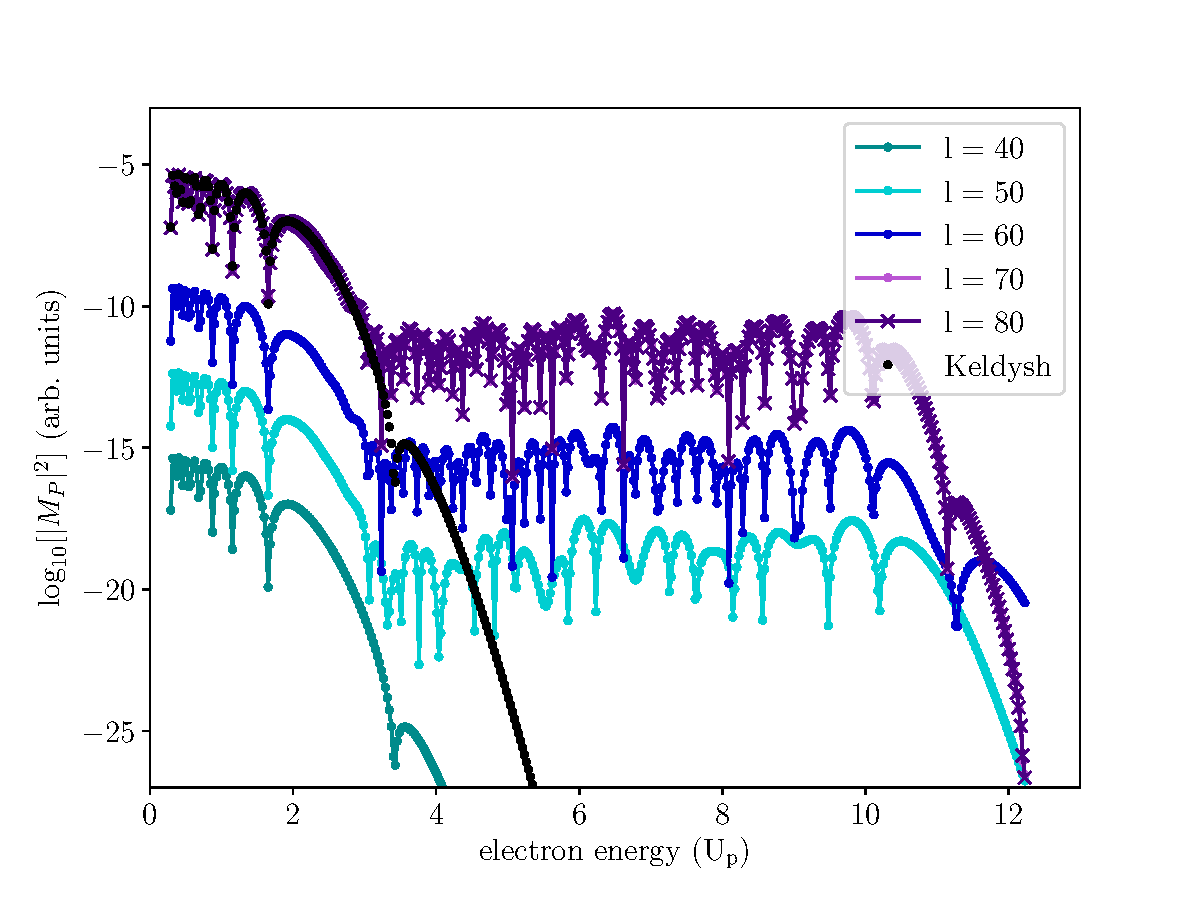
\includegraphics[width=0.75\textwidth]
                  {figures/ch_ATI_SFA/1b1/l40to80n512WP50PG25MR35vsKeldysh.pdf}
  \caption{ATI spectrum for the $1b_{1}$ MO of H$_{2}$O by a linearly
    polarized field with laser intensity of $10^{15}\ \rm{W/cm^{2}}$
    with $\hbar\omega = 1.58\ \rm{eV}$ in terms of an increasing
    Bessel order, $l$, as a function of the electron energy (in
    colour). The result from the standard Keldysh approximation is
    shown as the black dotted line.}
  \label{fig:1b1_spectrum}
\end{figure}

\begin{figure}
  \centering
  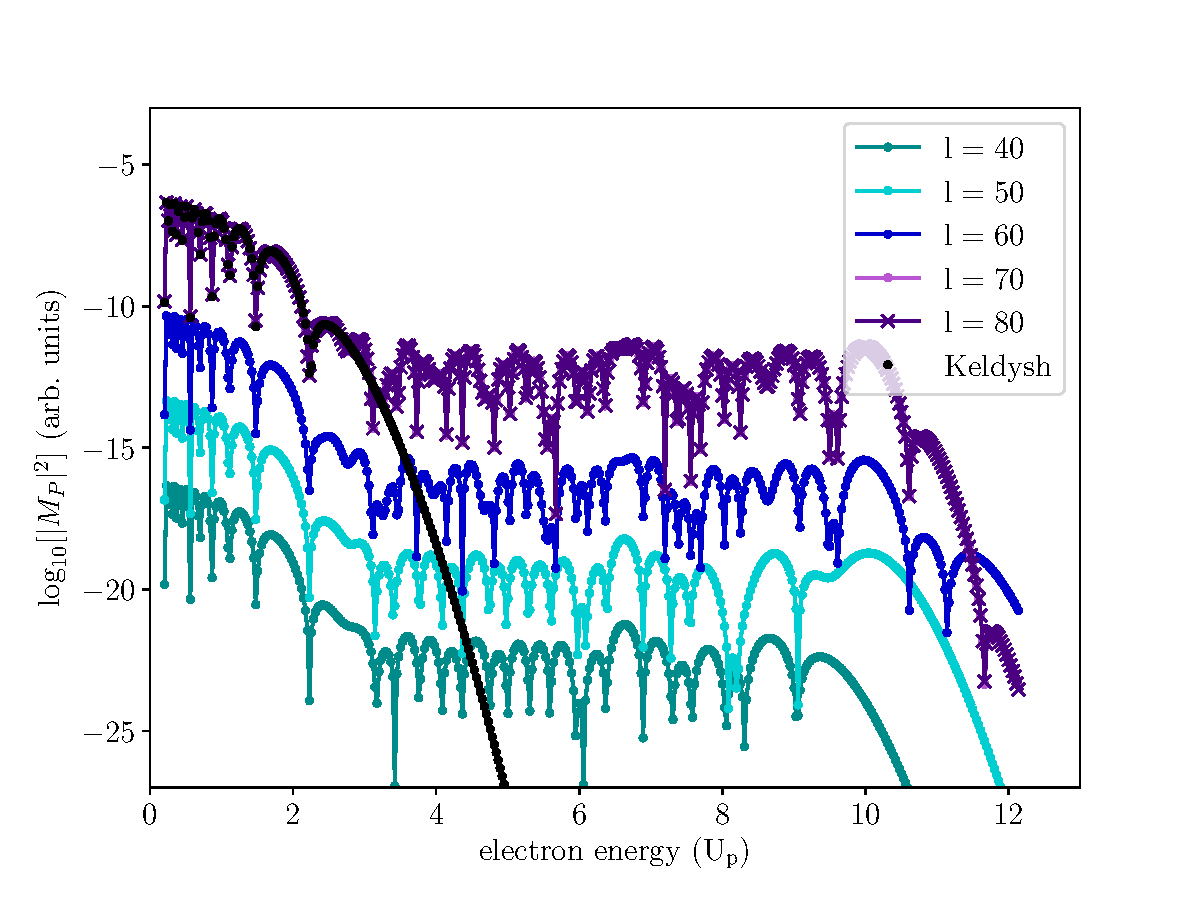
\includegraphics[width=0.75\textwidth]
                  {figures/ch_ATI_SFA/1b2/l40to80n512WP50PG25MR35vsKeldysh.pdf}
  \caption{ATI spectrum for the $1b_{2}$ MO of H$_{2}$O by a linearly
    polarized field with laser intensity of $10^{15}\ \rm{W/cm^{2}}$
    with $\hbar\omega = 1.58\ \rm{eV}$ in terms of an increasing
    Bessel order, $l$, as a function of the electron energy (in
    colour). The result from the standard Keldysh approximation is
    shown as the black dotted line.}
  \label{fig:1b2_spectrum}
\end{figure}

%As mentioned above

% more thorough description of the molecular orbital is needed



%%% Local Variables:
%%% mode: latex
%%% TeX-master: "thesis"
%%% End:
